\documentclass[
	12pt,				% tamanho da fonte		
	oneside,
	a4paper,			% tamanho do papel.
	chapter=TITLE,
	%sumario=tradicional,
	english,			% idioma adicional
	brazil,				% idioma principal do documento
	]{abntex2}

% ---
% PACOTES
% ---
\usepackage{lmodern}			% Usa a fonte Latin Modern
\usepackage[T1]{fontenc}		% Selecao de codigos de fonte.
\usepackage[utf8]{inputenc}		% Codificacao do documento (conversão automática dos acentos)
\usepackage{indentfirst}		% Indenta o primeiro parágrafo de cada seção.
\usepackage{color}				% Controle das cores
\usepackage{graphicx}			% Inclusão de gráficos
\graphicspath{{figuras/},{figuras/Intro/},{figuras/CAP2/},{figuras/CAP3/},{figuras/CAP4/},{figuras/CAP5/}}
\usepackage{microtype} 			% para melhorias de justificação
\usepackage{booktabs}
\usepackage{float} 				% Set posição da figura
\usepackage[bottom]{footmisc} 
\usepackage{subfig} 			% Inserir subfiguras
\usepackage[table,xcdraw]{xcolor} 	% Cor de preenchimento das tabelas
\usepackage{multirow} 			%mesclar cel em tabelas
\usepackage{verbatim}			%Inserir codigos fontes e comentários em massa
\usepackage[brazilian,hyperpageref]{backref}
\usepackage[alf]{lib/abntex2cite}
\usepackage{lipsum}				% para geração de dummy text
\usepackage{amsmath}
\usepackage[bottom]{footmisc}
\usepackage{footnote}
%\usepackage{fnpos}
%\usepackage{ftnxtra}
\usepackage{listings} 			%Inserir códigos fontes
\usepackage{rotating} 			%Rotação de páginas
\usepackage{placeins}			% Forçar o posicionamento da figura
\usepackage[top=3cm, bottom=2cm, left=3cm, right=2cm]{geometry} % Margens


% ---
% Informações de dados para CAPA e FOLHA DE ROSTO
% ---

\titulo{{\normalfont \textbf{Título do seu Trabalho}}}
\autor{Jonathan da Silva Braga}
\local{Natal -- RN}
\data{Dezembro de 2017}
\instituicao{
  Universidade Federal do Rio Grande do Norte -- UFRN
  \par
  Departamento de Engenharia de Computação e Automação -- DCA
  \par
  Curso de Engenharia Mecatrônica

}
\tipotrabalho{Relatório técnico}

\preambulo{Trabalho de Conclusão de Curso de Engenharia Mecatrônica da Universidade Federal do Rio Grande do Norte, apresentado como requisito parcial para a obtenção do grau de Bacharel em Engenharia Mecatrônica
\newline 
\newline 
Orientador: John Doe}

% Configurações de aparência do PDF final
% alterando o aspecto da cor azul
\definecolor{blue}{RGB}{41,5,195}
% informações do PDF
\makeatletter
\hypersetup{
     	%pagebackref=true,
		pdftitle={\@title}, 
		pdfauthor={\@author},
    	pdfsubject={\imprimirpreambulo},
	    pdfcreator={LaTeX with abnTeX2},
		pdfkeywords={abnt}{latex}{abntex}{abntex2}{relatório técnico}, 
		colorlinks=true,       		% false: boxed links; true: colored links
    	linkcolor=black,          	% color of internal links
    	citecolor=black,        		% color of links to bibliography
    	filecolor=magenta,      		% color of file links
		urlcolor=blue,
		bookmarksdepth=4
}
\makeatother
% Espaçamentos entre linhas e parágrafos 
\setlength{\parindent}{1.25cm} % Tamanho do parágrafo
\setlength{\parskip}{0.2cm}	% Controle do espaçamento entre um parágrafo e outro

%\onelineskip % Controle do espaçamento entre um parágrafo e outro

\makeindex % compila o indice

% Início do documento
% ----
\begin{document}

% Seleciona o idioma do documento (conforme pacotes do babel)
%\selectlanguage{english}
\selectlanguage{brazil}

% Retira espaço extra obsoleto entre as frases.
\frenchspacing 

% ----------------------------------------------------------
% ELEMENTOS PRÉ-TEXTUAIS
% ----------------------------------------------------------
\pretextual

% Capa
\imprimircapa

% Folha de rosto
\imprimirfolhaderosto

% Inserir folha de aprovação
\begin{folhadeaprovacao}
	
	\begin{center}
		{\ABNTEXchapterfont\large\imprimirautor}
		
		\vspace*{\fill}\vspace*{\fill}
		\begin{center}
			\ABNTEXchapterfont\bfseries\Large\imprimirtitulo
		\end{center}
		\vspace*{\fill}
		
		\hspace{.45\textwidth}
		\begin{minipage}{.5\textwidth}
			\imprimirpreambulo
		\end{minipage}%
		\vspace*{\fill}
	\end{center}
	
	Banca Examinadora do Trabalho de Conclusão de Curso	
	
	\setlength{\ABNTEXsignwidth}{14cm}
	\assinatura{\textbf{Prof. Dr. Carlos Manuel Dias Viegas - Orientador}} 
	\assinatura{\textbf{Prof. Dr. Danilo Curvelo de Souza}}
	\assinatura{\textbf{Prof. M.Sc. Sérgio Natan Silva}}

	\vspace{1.5cm}
	
	\begin{center}
		\vspace*{0.5cm}
		{\large\imprimirlocal}
		\par
		{\large\imprimirdata}
		\vspace*{1cm}
	\end{center}
	
\end{folhadeaprovacao}

% Dedicatória
\begin{dedicatoria}
	\vspace*{\fill}
	\centering
	\noindent
	\textit{Escreva aqui sua dedicatórss}
	 \vspace*{\fill}
\end{dedicatoria}

% Agradecimentos
\begin{agradecimentos}
Escreva aqui seus agradecimentos.

\end{agradecimentos}

% ---
% Epígrafe
% ---
\begin{epigrafe}
	\vspace*{\fill}
	\begin{flushright}
		\textit{``Feliz o homem que encontrou a sabedoria e alcançou o entendimento,\\
			porque a sabedoria vale mais do que a prata, \\
			e dá mais lucro que o ouro."\\
			(Bíblia Sagrada, Provérbios 3, 13-14)}
	\end{flushright}
\end{epigrafe}

% RESUMO
% resumo na língua vernácula (obrigatório)
\setlength{\absparsep}{18pt} % ajusta o espaçamento dos parágrafos do resumo
\begin{resumo}

Este trabalho consiste no desenvolvimento de um sistema domiciliar de monitoramento de energia elétrica, em tempo real e totalmente customizável.
Tem como proposta um dispositivo e um sistema que juntos somam a nova realidade de meios para a economia de energia.
O equipamento tem como base a plataforma de prototipagem NodeMCU que possui o microcontrolador ESP8266 acoplado em seu circuito integrado,
o circuito que é controlado pelo NodeMCU possui um sensor de corrente que afere o consumo em tempo real de um dispositivo e, através
do envio desses dados a um servidor onde possui comunicação com um agente consumidor é possível acompanhar todo o consumo de energia elétrica em tempo real.
O intuito é que o constante monitoramento possa trazer uma conscientização da economia de energia.
 
 \noindent
 \textbf{Palavras-chaves}: Economia de energia. Monitoramento. Eficiência Energética. IoT. 
\end{resumo}
% ---
% resumo em inglês
\begin{resumo}[Abstract]
	\begin{otherlanguage*}{english}	
	
	This work consists of the development of a real-time home monitoring system for electricity, which is fully customizable. It proposes a device and a system that together add the new reality of means for energy saving. The equipment is based on the NodeMCU prototyping platform that has the ESP8266 microcontroller coupled to its integrated circuit, the circuit that is controlled by the NodeMCU has a current sensor that measures the real time consumption of a device and, by sending this data to a server where you have communication with a consumer agent it is possible to monitor all the consumption of electricity in real time. The intention is that constant monitoring can bring an awareness of energy savings.
	
	\vspace{\onelineskip}
	\noindent 
	\textbf{Keywords}: Energy saving. Monitoring. Energy Efficiency. IoT
	\end{otherlanguage*}
\end{resumo}

% ---
% inserir lista de ilustrações
\pdfbookmark[0]{\listfigurename}{lof}
\listoffigures*
\cleardoublepage

% inserir lista de tabelas
\pdfbookmark[0]{\listtablename}{lot}
\listoftables*
\cleardoublepage

% inserir lista de abreviaturas e siglas
\begin{siglas}
\item[HTML]   \textit{HyperText Markup Language}
\item[CSS]	  \textit{Cascading Style Sheets}
\item[API]    \textit{Application Programming Interface}
\item[HTTP]   \textit{HyperText Transfer Protocol}
\item[TCP]    \textit{Transmission Control Protocol}
\item[JSON]   \textit{JavaScript Object Notation}
\item[REST]   \textit{Representational State Transfer}
\item[EPE]    \textit{Empresa de Pesquisa Energética}
\item[ANEEL]  \textit{Agência Nacional de Energia Elétrica}
\item[CEMIG]  \textit{Comapanhia Energética de Minas Gerais}
\item[SIN]    \textit{Sistema Interligado Nacional}
\item[IBGE]    \textit{Instituto Brasileiro de Geografia e Estatística}
\end{siglas}

% inserir lista de símbolos
\begin{simbolos}
  \item[$ \Gamma $] Letra grega Gama
  \item[$ \Lambda $] Lambda
  \item[$ \zeta $] Letra grega minúscula zeta
  \item[$ \in $] Pertence
\end{simbolos}

% inserir o sumario
\pdfbookmark[0]{\contentsname}{toc}
\tableofcontents*
\cleardoublepage

\textual

% Capitulo 1: Introdução
\chapter[Introdução]{Introdução}
\label{ch:introdução}
A eletricidade se tornou um pilar central na atualidade, sendo uma das principais fontes de força, calor e luz utilizada no  mundo. Entrantando com o
crescente consumo de energia elétrica nos últimos tempos, a demanda por produção da mesma teve um crecismento significativo, trazendo consigo 
impactos ambientais e econômicos. O Brasil por mais que possua em seu território grandes possibilidade para a construção de fontes de obtenção de energia, não
está isento do problema da alta demanda por energia elétrica. Problema que se agravou em 2015 quando o país começou a passar por
uma crise hídrica.

Como a \autoref{fig:rede_convencional} mostra, a maior parte da energia elétrica gerada no Brasil é por meio de hidroelétricas, essa dependência
energetica junto com a crise hídrica que o país sofreu cuminou em uma política de racionamento e aumento dos impostos - taxa inflacionária no
consumo de energia elétrica - que impactou diretamente a vida de cada cidadão brasileiro, trouxe consequências, como o aumento do 
custo da energia elétrica. Segundos dados (G1, 2016) entre 2015 e 2016 a crise hídrica no Brasil não interferiu apenas na conta de luz mas trouxe
um aumento na inflação do país.

% sustentabilidade


% JONATHAN aqui seu capítulo introdutório. Ele pode conter figuras, tabelas e subseções. Exemplo de uma citação indireta \cite{yu2011new}, e da \autoref{fig:rede_convencional}. Imagens do autor, tem na fonte o texto "Elaborado pelo autor".

\begin{figure}[h!]
	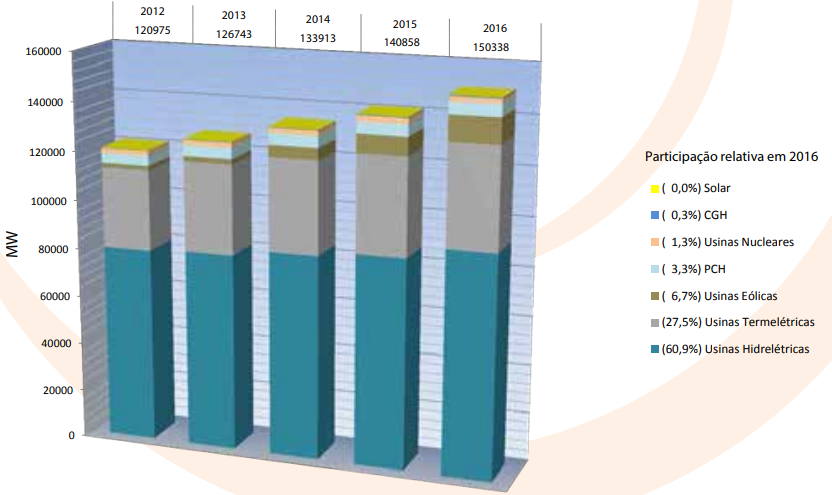
\includegraphics[width=0.9\textwidth, keepaspectratio=true]{forma_energia}
	\centering
	\caption[Capacidade de instalada de geração elétrica no Brasil (MW)]{Capacidade de instalada de geração elétrica no Brasil (MW)}
	\fonte{\cite[p. 57]{epe-anuario}.}
	\label{fig:rede_convencional}
\end{figure}
\FloatBarrier

%%%%%%%%%%%%%%%%%%%%%%%%%%%%%%%%%%%%%%%%%%%%%%%%%%%%%%%%%%%%%%%%%%%%%%%%%%%%%%%%%%%%%%%%%%%%%%%%%%%%%%%%%%%

O Consumo de energia elétrica é um dos principais indicadores de desenvolvimento e de qualidade de vida 
de um país. Esse índice é tão importate que reflete diretamente no rítimo de vida de uma populção, pois mostra
se as atividades industriais de uma nação está ou não em um bom rítimo e pode detectar se o comércio está em alta,
devido aos bens e serviços que o povo adiquiriu. Porém um crescimento desordenado na população e um crescimento
exponencial no consumo de enérgia pode acarretar em problemas para um determinado país.
Analisando os dados \cite{epe-balanco-final}, o consumo de energia
elétrica no Brasil vem crescendo ao longo dos anos, o brasileiro vem consumindo mais energia elétrica, nos últimos
35 anos teve um crescimento médio de 6,72\% dessa demanda, após a crise que o Brasil sofreu entre os anos 2002 e 2005 houve um crescimento
de 4,91\% na demanda energética do país. A \autoref{fig:consumo_energia_total} nos mostra bem o cenário de crise energética que o Brasil vinha
passando ao longo dos anos, até 2008 o país consumia mais do que produzia.

\begin{figure}[h!]
	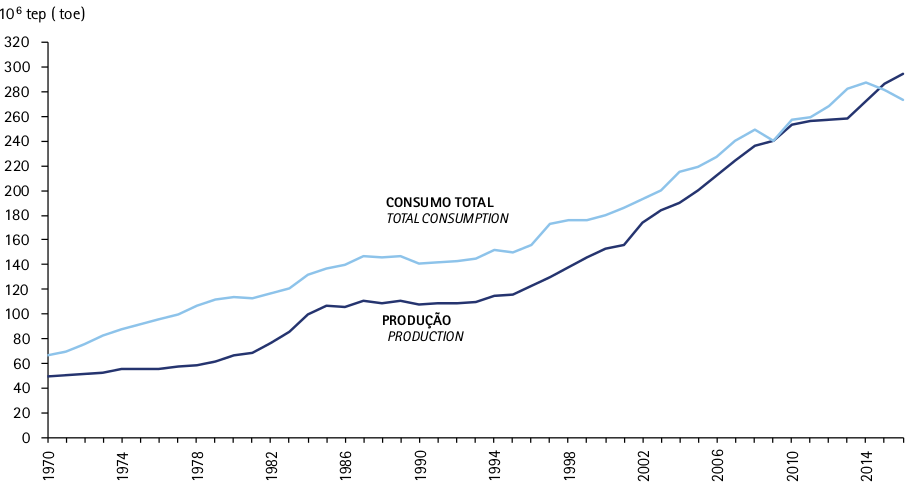
\includegraphics[width=0.85\textwidth, keepaspectratio=true]{consumo_energia_total}
	\centering
	\caption[Estrutura do Consumo de fontes primárias]{Estrutura do Consumo de fontes primárias}
	\fonte{\cite[p. 43]{epe-balanco-final}.}
	\label{fig:consumo_energia_total}
\end{figure}
\FloatBarrier

O governo brasileiro tomou algumas medidas estratégicas para poder acompanhar a crescente demanda por energia elétrica, constituiu o planejamento
da construção de mais de 80 usinas até 2020, hidroelétricas, temoelétricas e até usina nuclear. Um grande problema desse planjamento que o gorverno
fez são os inumeros impactos ambientais e econômicos, um exemplo prático é a usina de de Belo Monte - Rio Xingu, Pará - obra que foi planejada
para ser a quarta maior hidroelétrica do mundo, a maior do Brasil, com capacidade habastecer 40\% das recidências, foi orçada em R\$ 30 bilhões
deveria ter seu início de operação no segundo semestre de 2015 mas até os dias atuais não entrou em funcionamento. Vale salientar que a construção
trouxe o desmatamento de áreas indígenas, alagamentos permanentes, comprometimento da fauna e flora e aumento da dificuldade dos transportes fluviais
de comunidades ribeirinhas.

Analisando a grande demanda energetica que o brasileiro vem requerindo e levando em conta as consquências negativas do planejamento das 80 usinas,
surgi uma questão bastante recorrente: - "O que fazer? Constuir usinas mesmo sabendo dos impactos negativos que podem surgir, ou não construí-las e
aumentar a tarifação pelo consumo de energia visando diminuir o consumo?" - A resposta para essas e outras questões que podem aparecer não são fáceis.
Entretanto o governo brasileiro optou por deixar o consumo de energia elétrica mais caro, principalmente nos horários de pico. A evolução da tarifa,
pode ser observada na \autoref{evolucao-tarifa}


\begin{table}[!ht]
	\centering
	\begin{tabular}{lcccc}
	\hline
	\textbf{Ano} & \multicolumn{1}{l}{\textbf{1º Trimestre}} & \multicolumn{1}{l}{\textbf{2º Trimestre}} & \multicolumn{1}{l}{\textbf{3º Trimestre}} & \multicolumn{1}{l}{\textbf{4º Trimestre}} \\ \hline
	\rowcolor[HTML]{DDDDDD} 
	2013         & 120,8                                     & 117,1                                     & 114,5                                     & 116,1                                     \\
	2014         & 121,1                                     & 127,6                                     & 134,4                                     & 141,9                                     \\
	\rowcolor[HTML]{DDDDDD} 
	2015         & 154,2                                     & -                                         & -                                         & -                                        
	\end{tabular}
	\caption{Evoluçao dos custos de energia elétrica em R\$/MWh}
	\fonte{\cite[p. 1]{evolucao-tarifa-ref}}
	\label{evolucao-tarifa}
\end{table}

Uma medida totalmente cabível que ainda é desconhecida por alguns brasileiros é a chamada "\textit{exposição da informação}", deixando sempre bem claro 
quanto o consumidor tem gastado ou consumindo ao longo do mês em sua recidência, isso é possível graças a equipamentos que estão sempre monitorando
a rede elétrica.Segundo uma pesquisa realizada pela Associação Brasileira das Empresas de Serviços de Conservação de Energia, em seis anos o Brasil 
desperdiçou o equivalente a 250GWh em energia o que equivale a R\$62 bilhões, desperdíciu que se deu justamente a tamanha falta de infomação que 
o consumidor tem, se ao saber o quanto tem consumido ou gastado em tempo real o consumidor poderia se prevenir dos desperdícios. 

\subsection[\textit{Setor Energético Brasileiro}]{\textit{Setor Energético Brasileiro}}\label{seb}
Ao passar dos anos o Brasil vem mostrando cada vez mais o seu potencial na produão de energia, o território brasileiro possibilita as várias formas
de obtenção da eletricidade. Analisando os dados \cite[p.29]{epe-anuario-2015} e comparando com a \autoref{cap_ele} nota-se que o Brasil subiu duas
posoções no \textit{Rank} de geração de energia elétrica, isso é reflexo do aumentou da capicidade de produção de energia que chegou na marca de 8,39\%.

\begin{table}[!ht]
	\centering
	\begin{tabular}{lccccc}
		\rowcolor[HTML]{9B9B9B} 
		\multicolumn{1}{c}{\cellcolor[HTML]{9B9B9B}} & {\color[HTML]{FFFFFF} \textbf{2010}} & {\color[HTML]{FFFFFF} \textbf{2011}} & {\color[HTML]{FFFFFF} \textbf{2012}} & {\color[HTML]{FFFFFF} \textbf{2013}} & \multicolumn{1}{l}{\cellcolor[HTML]{9B9B9B}{\color[HTML]{FFFFFF} \textbf{2014}}} \\ \hline
		\textbf{Mundo}                               & \multicolumn{1}{l}{\textbf{5080,6}}  & \multicolumn{1}{l}{\textbf{5305,0}}  & \multicolumn{1}{l}{\textbf{5514,6}}  & \multicolumn{1}{l}{\textbf{5736,2}}  & \multicolumn{1}{l}{\textbf{6038,7}}                                              \\ \hline
		\rowcolor[HTML]{DDDDDD} 
		China                                        & 971,8                                & 1069,5                               & 1154,6                               & 1267,7                               & 1399,5                                                                           \\
		Estados Unidos                               & 1039,1                               & 1051,3                               & 1063,0                               & 1060,1                               & 1074,6                                                                           \\
		\rowcolor[HTML]{DDDDDD} 
		Japão                                        & 284,9                                & 287,3                                & 293,3                                & 300,8                                & 313,4                                                                            \\
		Índia                                        & 213,1                                & 246,0                                & 260,3                                & 283,0                                & 310,8                                                                            \\
		\rowcolor[HTML]{DDDDDD} 
		Rússia                                       & 228,1                                & 231,6                                & 233,6                                & 235,2                                & 247,6                                                                            \\
		Alemanha                                     & 162,7                                & 167,5                                & 177,3                                & 186,1                                & 198,4                                                                            \\
		\rowcolor[HTML]{DDDDDD} 
		Canadá                                       & 132,3                                & 132,9                                & 130,7                                & 133,3                                & 136,8                                                                            \\
		Brasil                                       & 11,3                                 & 117,1                                & 121,0                                & 126,7                                & 133,9                                                                           
	\end{tabular}
	\caption{Capacidade instalada de geração elétrica no mundo, 2014 (GW)}
	\fonte{\cite[p. 29]{epe-anuario}}
	\label{cap_ele}
\end{table}

A maior produção de energia do Brasil provem das hidroelétricas, o país é referência mundial quando o assunto é obtenção de energia através de
usinas hidroelétricas - \autoref{cap_hidro} - isso é possível devido a sua alta concentração de rios de grande porte e ao grande volume de chuva
que alimenta e reforça o poderio hídrico do país. A energia que a usina hidroelétrica fornece é conseguida através da energia hidráulica que provém
do aproveitamento da força potencial e cinética das correntes de água,rio, mar. A água ao passar por tubulações com muita força e velociadade 
movimentas as turbinas fazendo com que elas girem em um velociadade suficiente para que os geradores acoplados nas turbinas, transformem energia
mecânica em energia elétrica, lembrando que a eficiência energética de uma usina hidroelétrica é de 65,2\%. Após esse longo processo a energia 
extraída é enviada para estações de tratamento e após essa etapa é enviada para a matriz energetica que fará a distribuião da energia extraída. 

\begin{table}[!ht]
	\centering
	\begin{tabular}{lccccl}
		\rowcolor[HTML]{9B9B9B} 
		\multicolumn{1}{c}{\cellcolor[HTML]{9B9B9B}} & {\color[HTML]{FFFFFF} \textbf{2010}} & {\color[HTML]{FFFFFF} \textbf{2011}} & {\color[HTML]{FFFFFF} \textbf{2012}} & {\color[HTML]{FFFFFF} \textbf{2013}} & {\color[HTML]{FFFFFF} \textbf{2014}} \\ \hline
		\textbf{Mundo}                               & \multicolumn{1}{l}{\textbf{903,9}}   & \multicolumn{1}{l}{\textbf{929,9}}   & \multicolumn{1}{l}{\textbf{957,5}}   & \multicolumn{1}{l}{\textbf{1000,4}}  & \textbf{1038,3}                      \\ \hline
		\rowcolor[HTML]{DDDDDD} 
		China                                        & 199,5                                & 214,6                                & 229,1                                & 258,9                                & 283,0                                \\
		Brasil                                       & 80,7                                 & 82,5                                 & 84,3                                 & 86,0                                 & 89,2                                 \\
		\rowcolor[HTML]{DDDDDD} 
		Estados Unidos                               & 78,8                                 & 78,7                                 & 78,7                                 & 79,2                                 & 79,7                                 \\
		Canadá                                       & \multicolumn{1}{l}{74,9}             & \multicolumn{1}{l}{75,4}             & \multicolumn{1}{l}{75,4}             & \multicolumn{1}{l}{75,4}             & 75,4                                
	\end{tabular}
	\caption{Capacidade instalada de geração hidrelétrica no mundo, 2014 (GW)}
	\fonte{\cite[p. 30]{epe-anuario}}
	\label{cap_hidro}
\end{table}

É do conhecimento de qualquer brasileiro que possua uma noção básica de geografia que a região norte é a região que possui a maior quantidade de rios,
essa noção pode levar uma conclusão errada - A região norte é a que mais produz energia - pois nem todo rio tem potencial para que uma hidroelétrica se instale.
Por sua vez as regiões sul e suldeste são as que mais necessitam de energia, devido a densidade populacional e a quantidade de insdutrias instaladas nas regiões.
A \autoref{pxcxge} externa essa problemática de uma manéira bem visível. Perceb-se que por exemplo a região sudeste é a que produz mais energia, porém é a que mais
gasta, sendo os gastos maiores do que os ganhos, já a região norte e nordeste são regiões que produzem mais do que gastam. Vendo esse total desequilíbrio
de geração e consumo de energia, surgiu a necessidade da criação do Sistema Interligado Nacional (SIN). O SIN é constituido por todas as regiões brasileiras
e é interconectado por meio de uma malha de trasmissão que propicia a transferência de energia entres os subsistemas, permitindo a obtenção de ganhos
sinérgicos e explora a diversidade entre os regimes hidrológicos e das bacias. A integração dos recursos de geração e transmissão permite o atendimento ao
mercado com segurança e economicidade.
\begin{table}[!ht]
	\centering
	\begin{tabular}{cccc}
		\hline
	\textbf{Região} & \textbf{População} & \textbf{Consumo em GW} & \textbf{\begin{tabular}[c]{@{}c@{}}Capacidade Instalada de \\ Geração Elétrica GW\end{tabular}} \\ \hline
		\rowcolor[HTML]{DDDDDD} 
		Norte           & 17.707.783         & 12,197                 & 25,484                                                                                          \\
		Nordeste        & 56.915.936         & 12,109                 & 29,803                                                                                          \\
		\rowcolor[HTML]{DDDDDD} 
		Sudeste         & 86.356.952         & 74,584                 & 44,810                                                                                          \\
		Sul             & 29.439.773         & 19,173                 & 31,681                                                                                          \\
		\rowcolor[HTML]{DDDDDD} 
		Centro-Oeste    & 15.660.988         & 5,634                  & 18,558                                                                                         
	\end{tabular}
	\caption{Relação População x Consumo por Região x Geração Elétrica por Região}
	\fonte{(IBGE\protect\footnotemark  e  EPE\protect\footnotemark)}
	\label{pxcxge}
\end{table}

\addtocounter{footnote}{-1}
\footnotetext{\cite{epe-balanco-final}}
\addtocounter{footnote}{1}
\footnotetext{\url{https://ww2.ibge.gov.br/home/estatistica/populacao/estimativa2009/estimativa.shtm}{}}

\subsection[\textit{Medição de Energia}]{\textit{Medição de Energia}}\label{med-energia}

Após enterder todo o funcionamento da geração e distribuição de energia no Brasil, é conveniente entender o processo de leitura do consumo de 
energia elétrica, assim como as questões que esse trabalho faz a respeito da eficácia. Tendo a possibilidade de atualizar esse sistema com novas 
tecnologias que proporcinam maior segurança e menores custos ao consumidor.

Os primeiros medidores de eletricidade foram utilizados na operação de lâmpadas em série, um vez que a tensão era constante, a corrente exigida
por cada lâmpada era conhecida e todas estavam ligadas no mesmo interruptor, os medidores foram suficientes apenas para medir o gasto das lâmpadas
em um tempo determinado, surgindo o termo - lâmpada-hora. Em 1872 o pesquisador Samuel Gardiner trouxe a toda a primeira patente sobre um contator 
de energia, que era formado por uma lâmpada acoplada a um contador de energia DC controlado por um relógio e um eletroímã, ao passar do tempo várias
outras patentes foram surgindo e tentando melhor o projeto de Samuel Gardiner, mas foi apenas em 1892 que que surgiu o primeiro medidor de watt-hora
com precisão e confiabilidade suficiente para aplicação em medição de consumo de energia. Criado por Thomas Duncan, inicialmente seu objetivo era a medição
de circuitos monofásicos, porém com o bom desempenho do aprelho modificações foram feitas para à medição de circuitos polifásicos de energia.

Atualmente a energia elétrica é quantificada através de um equipamento chamado medidor, que nos dias atuais a medição é feita em quilowatt-hora.
Os medidores da atualidade são caracterizados por padrões da norma NBR 14519, o grupo de medidor mais utilizado pelas concessionárias nas residências
é o grupo B. 

\begin{itemize}
	\item Grupo B \\
	É caracterizado por unidades consumidoras de baixa tensão, com tensões inferiores a 2,3KV. As unidades consumidores podem ser classificadas
	mediante a necessidade da concessionária responsável, geralmente o tipo B1 é residencial, tipo B2 são as residências rurais e estabelecimentos
	comerciais ou insdustriais são classificados como o tipo B3.
\end{itemize}

Estima-se que 92\% dos medidores em funcionamento são eletromecânicos, pois são de baixa custo e de boa qualidade, com o erro máximo de 2\% de seu valor
nominal de operação. Não ter um medidor em uma unidade consumidora pode gerar transtornos tanto para concessionário, pois não saberá o quanto deve cobrar ao 
consumidor, como para o dono do estabelecimento, pois não terá o aporte devido prestado pela concessionária de energia.

\subsection[\textit{Automação}]{\textit{Automação}}\label{automacao}
Mesmo com a grande evolução que os medidores eletromecânicos sofreram ao longo do tempo, os dispositivos ainda apresentam pontos frágeis, dando uma 
grande margem ao erro. A grande quantidade de peças mecânicas presente no medidor, faz com que o mesmo possua algumas limitações: interferência na
opreção na presença de corrente continua que causam deformações no fluxo magnético do leitor; diminuição da precisão quando são tratados de valores
muito baixos. Hoje em dia existe uma forte tendência a substitução desses medidores eletromeânicos por medidores eletrônicos, irá possibilitar além de uma
melhor precisão uma maior e melhor medição e até possibilitando uma leitura remota. Hoje no Brasil existe um projejto de lei (PL 2932/20015) que prevê
a substitução de medidores de consumo de energia eletromecânicos por medidores eletromecânicos inteligentes em até 15 anos após a aprovação da lei.

%%%%%%%%%%%%%%%%%%%%%%%%%%%%%%%%%%%%%%%%%%%%%%%%%%%%%%%%%%%%%%%%%%%%%%%%%%%%%%%%%%%%%%%%%%%%%%%%%%%%%%%%%%%%

A necessidade de contornar os desafios da crescente demanda energetica insentiva a busca por fontes alternativas e limpas de energia. O Brasil 
possui 42,30\% de fontes renováveis da sua matriz energetica e esse número deve aumentar até 2021 onde alcançará a marca de 85,00\% (as hidroelétricas
estão inclusas nesse meio), segundo o Ministério de Minas e Energia. No Plano Decemal de Expansão de Energia (PDE) 2020, o gorveno brasileiro
assume que a sustentabilidade é a chave mestra para a expenssão de atividades de geração de energia elétrica. A \autoref{fig:fonte_energia} mostra
que o Brasil vem investindo ao passar dos anos em fontes limpas de energias. Contudo também mostra que o Brasil ainda é muito dependente das 
hidrelétricas que apesar de ser uma fonte limpa e renovável traz malefícios como as grandes áreas alagadas em volta da represa, impactando no
ciclo de vida das espécies e obriga populaões ribeirinhas a migrarem, isso mostra que não basta apenas ter fontes limpas
e renováveis de energia, é necessário buscar melhorias como as Smart Grids e técnicas como de Smart metering.

\begin{figure}[h!]
	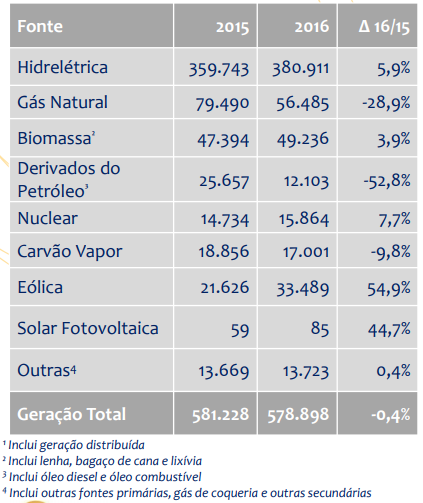
\includegraphics[width=0.7\textwidth, keepaspectratio=true]{fontes_energia}
	\centering
	\caption[Fontes de geração de energia elétrica (GWh)]{Fontes de geração de energia elétrica (GWh)}
	\fonte{\cite[p. 35]{epe-balanco}.}
	\label{fig:fonte_energia}
\end{figure}
\FloatBarrier

As chamadas redes inteligentes de transmissão e distribuição de energia, smart grid, tem como objetivo conectar unidades descentralizadas de geração
grande e pequena com o consumidor final. Assim nessa ideia o fluxo de energia se comunica de uma maneira bidirecional, a energia que é tradicionalmente
gerada e distribuidas pelas concessionárias poderá ser gerada e integrada as redes elétricas apartir de unidades consumidoras. O grande pilar dessa 
tecnologia são os sensores instalados ao longo da rede elétrica que constantemente estão enviando informações referente ao consumo a concessionária,
possibilitando um planejamento mais eficiente da rede. Aliado aos sensores na rede elétrica o consumidor recebe um medidor inteligente que também
é integrado com a concessionária em tempo real.

\begin{figure}[h!]
	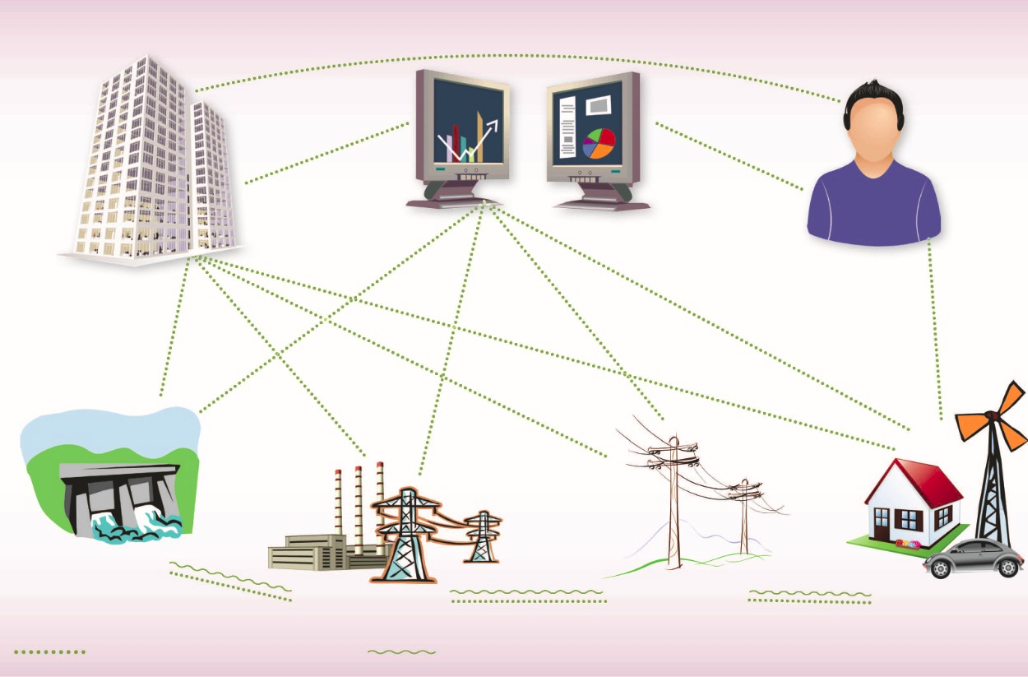
\includegraphics[width=0.7\textwidth, keepaspectratio=true]{rede_smartgrid}
	\centering
	\caption[Smart Grid,comunicação inteligente entre todos os usuários]{Smart Grid,comunicação inteligente entre todos os usuários}
	\fonte{\cite{smart-grid}.}
	\label{fig:rede_smartgrid}
\end{figure}
\FloatBarrier

O trabalho apresentará uma forma barata e eficiente de monitorar a energia elétrica de uma residência em tempo real, possibilitanto ao usuário
possuir informações valiosas a todo momento. O trabalho fará um paralelo com algumas possibilidades de medição de consumo e monitoramento
de energia, provando através da prática que é possível conscientizar o usuário do mau uso da energia elétrica.
Então a partir desse dispositivo será possível entender como e onde a energia está sendo gasta. O sistema também disponibilza de ferramentas para que 
caso o utente possua o conhecimento necessário o mesmo venha a modificar ou aprimorar o gerenciamento de energia. O sistema nomeado de \textit{power monitor}
traz consigo uma nova forma de enxergar o consumo dos aparelhos presentes em uma residência, trocando o quilowatt-hora pela moeda de circulação no país,
o real, tal mudança é o principal fator de consientização, pois aproxima o consumidor dos gastos energéticos.


\section{Motivação}
A conjuntura do cenário energético atual do Brasil, junto com a crise em vários setores e principalmente no setor
energético do país e a falta de transparência na informação levada ao usuário foi o que motivou este trabalho. Hoje se vive em uma realidade onde
ter informação em tempo real do consumo de energia em um estabeleciento é muito difícil, pois os equipamentos que proporcionam esse tipo de informação
não são acessíveis a todos os brasileiros, apenas companhias de energia ou pessoas com alto grau de estudo conseguem manusear ou entender o dados
fornecidos por esse tipo de equipamento. Toda essa privação da informação traz consequências, uma delas é o descaso do brasileiro em relação ao
racionamento de energia elétrica, como já foi citado no trabalho o Brasil em seis anos desperdiçou o equivalente a R\$ 62 bilhões, motivo que se 
dá a falta de conscientização do consumidor. Trazer uma forma com que consumo de energia elétrica, conta de luz, fique mais fácil e simples de se entender
e acompanhar é o que o sistema \textit{power monitor} fará.   

\section{Objetivos}
A objetivo existente neste trabalho é da conscientização do consumidor em relação aos gastos energéticos presentes em sua residência. Percebendo o
atual cenário brasileiro de total falta de informação em relação ao consumo em tempo real de energia, junto com o período em que o país 
passou de crise hídrica e energética, este trabalho propõe uma alternativa simples e barata onde qualquer brasileiro independente do grau de 
escolaridade ou classe social poderá acompanhar o consumo de energia elétrica de sua residência de uma maneira mais fácil e direta. O \textit{power monitor}
é composto por elementos de \textit{software} e \textit{hardware} que gerenciam automaticamente todos os dispositivos cadastrados presentes em uma
residência, esse gerenciamento se deve ao conjunto formado pelo servidor \textit{web} que é responsável por enviar e receber informações ao \textit{hardware} e
a interface \textit{web}, juntamento com o banco de dados que é responsável por guardar todas as informações coletadas pelo \textit{hardware} e a interface
\textit{web} tem o papel de agente consumidor de todos os dados e tratará as informações da melhor forma possível.


\section{Estrutura do Trabalho}
Este trabalho foi desenvolvido no intuito de apresentar um sistema para o monitoramento de energia e conscientização do usuário em relação aos 
gastos energéticos presentes em sua residência. O trabalho foi estruturado para que se possa mostrar nos próximos capítulos os seguintes conteúdos:
\begin{itemize}
	\item Capítulo 2: Embasamento Teórico - Descrição das tecnologias utilizadas neste trabalho;
	\item Capítulo 3: Desenvolvimento - Será descrita as etapas de implementação do projeto, desde uma visão geral do funcionamento a comunicação entre \textit{hardware} e servidor \textit{web};
	\item Capítulo 4: Conclusão - Conclusão e trabalhos futuros;
\end{itemize}

% Capitulo 2
\chapter[Embasamento Teórico]{Embasamento Teórico}
\label{ch:cap2}
O \textit{Power Monitor} surgiu da necessidade da conscientização do gasto energético e da melhor compreensão da conta de luz. Baseado nesse conceito,
foi desenvolvido um \textit{software} que permite uma fácil comunicação com qualquer equipamento construído que tenha a finalidade de monitorar a energia elétrica e um \textit{hardware} para demonstração
da comunicação entre ambos.
O sistema traz uma forma mais fácil e próxima do consumidor final de se quantificar a energia elétrica consumida em um estabelecimento. No lugar do quilowatt-hora, medida usada atualmente,
o \textit{software} propõe mensurar o gasto energético em reais (R\$), trazendo a realidade do consumo mensal.

Este capítulo trará os conceitos essenciais para o entendimento do trabalho, descrevendo todas as tecnologias utilizadas no desenvolvimento 
do \textit{Power Monitor}.

\section[\textit{Ferramentas e linguagens}]{\textit{Ferramentas e linguagens}}\label{ferramenta-linguagem}
No decorrer do desenvolvimento do \textit{software} fez-se uso de algumas tecnologias e linguagens de programação que serão descrita a seguir.
\subsection[\textit{Node.js}]{\textit{Node.js}}\label{node}
Node.js é um \textit{framework}, interpretador do código JavaScript (\autoref{js}), com o foco do uso da linguagem do lado do cliente para servidores. Com um objetivo simples
que é ajudar desenvolvedores na criação de aplicações de alta escalabilidade, com códigos capazes de administrar e manipular várias conexões simultaneamente
em um único servidor. O \textit{Node.js} é baseado na \textit{runtime} V8 \textit{JavaScript Engine}. Foi desenvolvido por Ryan Danhl em 2009, e o seu desenvolvimento
é mantido pela fundação \textit{Node.js} e \textit{Linux Foundation} \cite{ref-nodejs}. 
\subsection[\textit{JavaScript}]{\textit{JavaScript}}\label{js}
JavaScript é uma linguagem de programação interpretada de alto nível, juntamente com HTML e CSS é uma das linguagens mais utilizadas no mundo \textit{web}.
Após o uso da linguagem as páginas \textit{web} começaram a ter uma maior interatividade com o usuário. A grande maioria dos \textit{browsers} tem um
mecanismo de compilação dedicado para o JavaScript \cite{ref-js}. Por ser uma linguagem multi-paradigma o JavaScript suporta paradigmas funcionais, orientados a eventos 
e até mesmo paradigmas de orientação a objeto.
Inicialmente era usada apenas no lado do cliente em \textit{web browsers}, mas atualmente está presente em vários outros tipos de \textit{softwares} incluindo
servidores - como já foi discutido na \autoref{node} - \textit{databases} e até sistemas \textit{desktop} como os leitores de PDF, programas de música e recentemente
vem ganhando espaço no desenvolvimento de aplicativos para celular \cite{ref-jsmobile}.

\subsection[\textit{WebSocket}]{\textit{WebSocket}}\label{websocket}
A ideia da tecnologia surgiu da problemática onde as comunicações entre servidor e aplicação eram baseadas na sobrecarga do HTTP, que não é indicado para aplicações
de baixa latência. O WebSocket pode ser definido como uma API que estabelece a conexão entre aplicação e servidor. Resumidamente é uma conexão, baseada no protocolo TCP, persistente
entre servidor e cliente onde ambas as partes podem enviar ou receber informações. A forma como a conexão acontece é simples:
o cliente e o servidor antes de tudo devem negociar o \textit{handshake}, que segundo \cite{ref-handshake} é o precesso pelo qual duas máquinas afirmam uma a outra que a reconheceu e está pronta para iniciar a comunicação.
No momento em que a negocição é confirmada a conexão é establecida, criando um canal de comunicação bidirecional. A \autoref{fig:websocket-diagram} retrata o cenário descrito.

\begin{figure}[h!]
	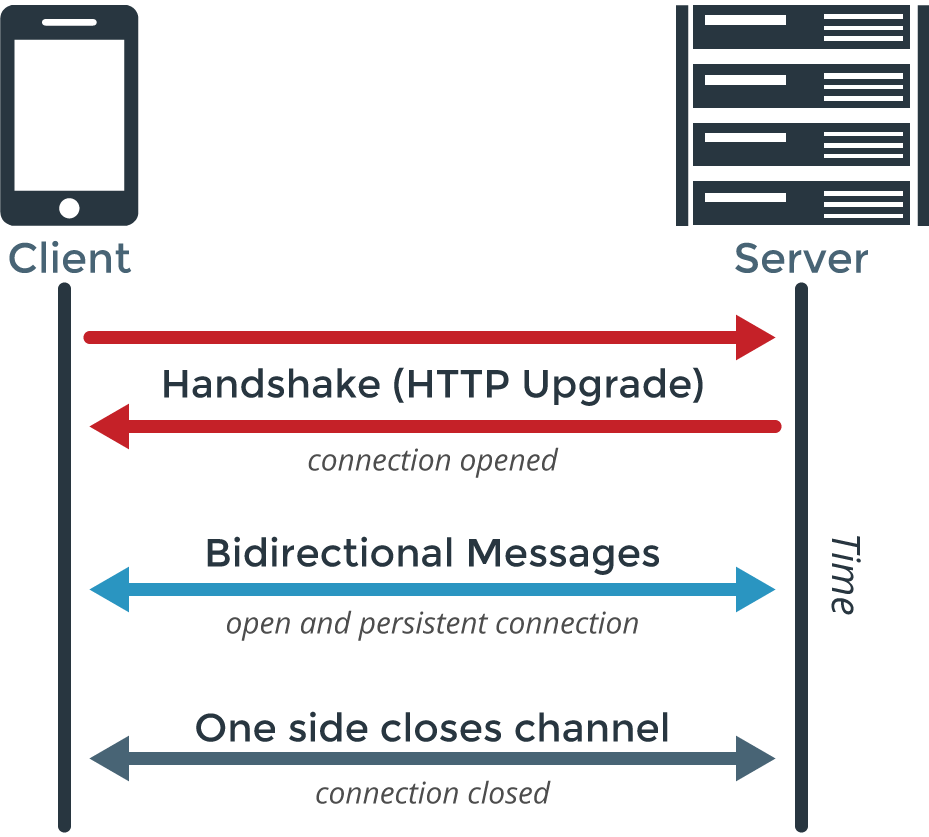
\includegraphics[width=0.45\textwidth, keepaspectratio=true]{websockets-diagram}
	\centering
	\caption[Diagrama de conexão via websocket]{Diagrama de conexão via websocket}
	\fonte{\url{https://www.pubnub.com/learn/glossary/what-is-websocket/}{}}
	\label{fig:websocket-diagram}
\end{figure}
\FloatBarrier


\subsection[\textit{SQL}]{\textit{SQL}}\label{sql}
Structured Query Language, ou comumente conhecida como SQL é uma linguagem padrão de banco de dados. 
Diferentemente das outras linguagens de banco de dados a consulta em SQL especifica a forma do resultado e não o caminho para chegar nele. Uma outra
grande diferença é que a linguagem SQL é declarativa diferindo mais uma vez das outras linguagens que por sua vez são procedurais \cite{ref-sqlhisto}.

O MySQL é um sistema de gerenciamento de banco de dados que utiliza a linguagem SQL. Atualmente é o sistema mais popular em gerenciamento de 
banco de dados. Sua rápida popularização deve-se a fácil comunicação entre servidor e aplicação.

\subsection[\textit{Fritzing}]{\textit{Fritzing}}\label{fritzing}
O \textit{Fritzing} é uma iniciativa \textit{open source} que inicialmente foi
designada a desenvolvedores amadores que gostasse de tirar a sua ideia do papel. Em poucas palavras
a plataforma auxilia os desenvolvedores por meio de uma interface gráfica nas primeiras montagens com Arduino
ou outro microcontrolador, sua intuitiva interface proporciona ao usuário uma rápida montagem do circuito em protoboard. O \textit{software} vai além
e permite com que os desenvolvedores tenha uma visão tanto da protoboar, como do esquemático elétrico. 


\section[\textit{Componentes Físicos}]{\textit{Componentes Físicos}}\label{comp-fisico}
No decorrer do desenvolvimento do \textit{hardware} fez-se uso de alguns componentes eletrônicos e microcontrolador que serão descritos nessa seção.
\subsection[\textit{ESP8266}]{\textit{ESP8266}}\label{esp}
É um SOC que é produzido por um fabricante chinês - Espressif - que tem como principal vantagem a comunicação \textit{Wi-Fi} já integrada em seu circuito.
O chip teve seu auge em 2014 quando "estourou" na cultura \textit{maker} com o ESP-01 (\autoref{fig:esp8266}), essa placa permite que microcontroladores se conectem a uma rede
sem fio  fazendo conexões TCP/IP, tendo a capacidade de ser servidor ou cliente \cite{ref-esp8266h}.

\begin{figure}[h!]
	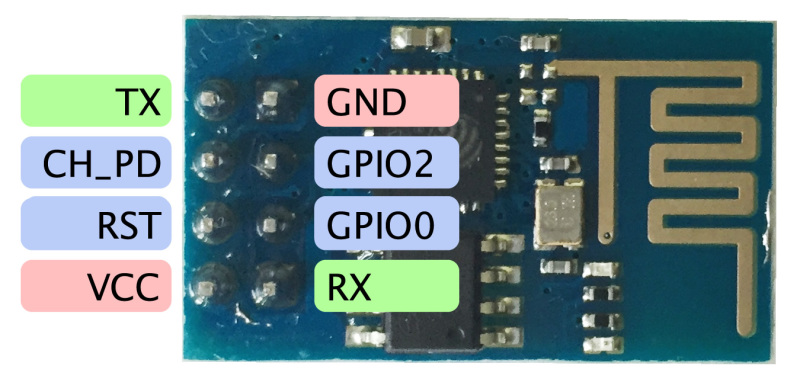
\includegraphics[width=0.3\textwidth, keepaspectratio=true]{esp8266}
	\centering
	\caption[ESP8266]{ESP8266}
	\fonte{\url{http://fabacademy.org/archives/2015/doc/images/esp-01.jpg}{}}
	\label{fig:esp8266}
\end{figure}
\FloatBarrier

O NodeMcu, \autoref{fig:nodemcu}, é uma plataformade de desenvolvimento \textit{open source}. Tem como principal linguagem de script Lua, foi construído sobre o SDK ESP8266.
A plataforma surgiu pouco tempo após o lançamento do ESP8266 (\autoref{esp}). A plataforma ganhou visibilidade, pois trazia um conjunto
de circuitos já previamente embutido que o ESP8266 por si só não proporcionava.

\begin{figure}[h!]
	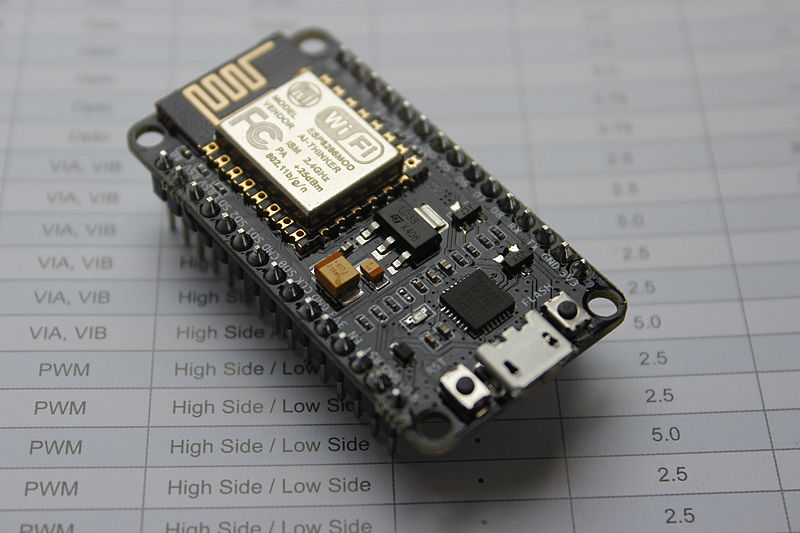
\includegraphics[width=0.4\textwidth, keepaspectratio=true]{nodemcu}
	\centering
	\caption[NodeMCU]{NodeMCU}
	\fonte{\url{https://upload.wikimedia.org/wikipedia/commons/7/7e/NodeMCU_DEVKIT_1.0.jpg}{}}
	\label{fig:nodemcu}
\end{figure}
\FloatBarrier

\subsection[\textit{Sensor de Corrente SCT 013-000}]{\textit{Sensor de Corrente SCT 013-000}}\label{sct}
O Sensor é um transformador de corrente para leituras não invasivas, possuindo um funcionamento similar a de um alicate amperímetro. Com a seguinte especificação
técnica: 
\begin{itemize}
	\item 100A no primário;
	\item Saída de 50mA no secundário;
	\item Temperatura máxima \ang{70}C;
	\item Temperatura mínima \ang{-25}C.
\end{itemize} 
Para realizar a leitura da corrente sem a necessidade de contato elétrico, o sensor de corrente alternada utiliza as propriedades 
magnéticas da corrente elétrica. O SCT, \autoref{fig:sct}, é um sensor do tipo Transformador de Corrente, que resumidamente é um conjunto de espiras que são
colocadas ao redor do condutor ao qual se quer medir a corrente. 

\begin{figure}[h!]
	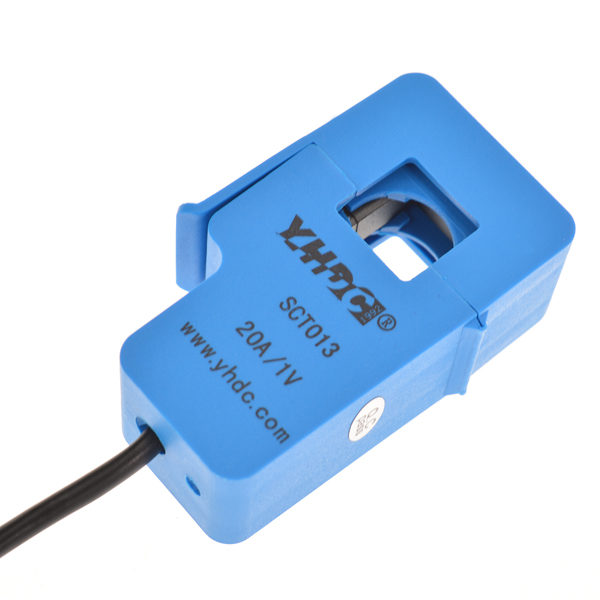
\includegraphics[width=0.3\textwidth, keepaspectratio=true]{sct}
	\centering
	\caption[SCT-013-000]{SCT-013-000}
	\fonte{\url{https://uploads.filipeflop.com/2017/07/1-34.jpg}{}}
	\label{fig:sct}
\end{figure}
\FloatBarrier


% Capitulo 3
\chapter[Desenvolvimento]{Desenvolvimento}
\label{ch:desenvolvimento}
O \textit{Power Monitor} surgiu da necessidade da conscientização do gasto energético e da melhor compreensão da conta de luz. Baseado nesse conceito,
foi desenvolvido um \textit{software} que permite uma fácil comunicação com qualquer equipamento construído que tenha a finalidade de monitorar a energia elétrica. 
O sistema traz uma forma mais fácil e próxima do consumidor final de quantificar a energia elétrica consumida em um estabelecimento. No lugar do Quilowatt-hora, medida que é usada atualmente,
o \textit{software} propõe mensurar o gasto energético em reais (R\$), trazendo a realidade do consumo mensal para mais próximo de cada brasileiro.

Nesse capítulo será mostrado todo o passo a passo para o desenvolvimento do \textit{software} e \textit{hardware}, juntamente com a comunicação 
entre ambos. 


\section[\textit{Visão Geral}]{\textit{Visão Geral}}\label{visal-geral}

Em resumo pode-se ter uma visão geral de como o ambiente - \textit{software} e \textit{hardware} - funciona observando a \autoref{fig:diagrama-vg}.
O sistema \textit{web} é responsável por fazer a comunicação entre o banco de dados e os dispositivos, já os eletrodomesticos são gerenciados
pelo ESP8266 que possui uma comunicação direta via \textit{websocket} com o servidor \textit{web}.

\begin{figure}[h!]
	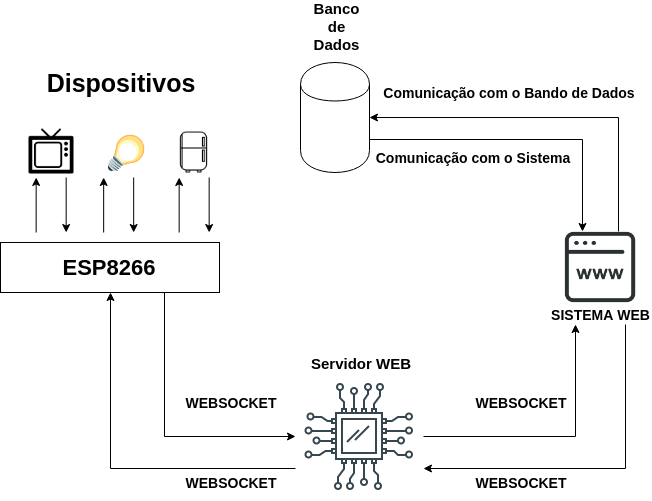
\includegraphics[width=0.7\textwidth, keepaspectratio=true]{diagrama-1}
	\centering
	\caption[Visão geral do ambiente]{Visão geral do ambiente}
	\label{fig:diagrama-vg}
\end{figure}
\FloatBarrier

\section[\textit{Software}]{\textit{Software}}\label{soft-sec}
O controle dos dispositivos de um cômodo, que estão interligados com o \textit{ESP8266} são controlados pelo \textit{software}. Dessa forma
todos os dispositivos que possuem comunicação com o microcontrolador e que estão cadastrados nos sistema podem ser controlados (Ligar/Desligar) e também
é possível ter um acompanhamento dos gastos.

O sistema possui uma interface \textit{web} que pode ser acessada por qualquer dispositivo que tenha acesso a internet e possua um 
\textit{browser}, como por exemplo: celulares, computadores, \textit{smart tv} etc. O \textit{software} possui uma interface de apenas um único usuário, ao acessar o sistema o usuário se depara com um
visual bem agradável e fácil de se usar. Logo ao entrar no sistema o utente se depara com a tela princiapl, \autoref{fig:principal-ft}, nela encontra-se
as principais informações que o usuário irá precisar, como também irá mostrar as opções de cadastrar um novo dispositivo, listar os dispositivos, cadastrar um novo cômodo,
listar um novo cômodo etc.

\begin{figure}[h!]
	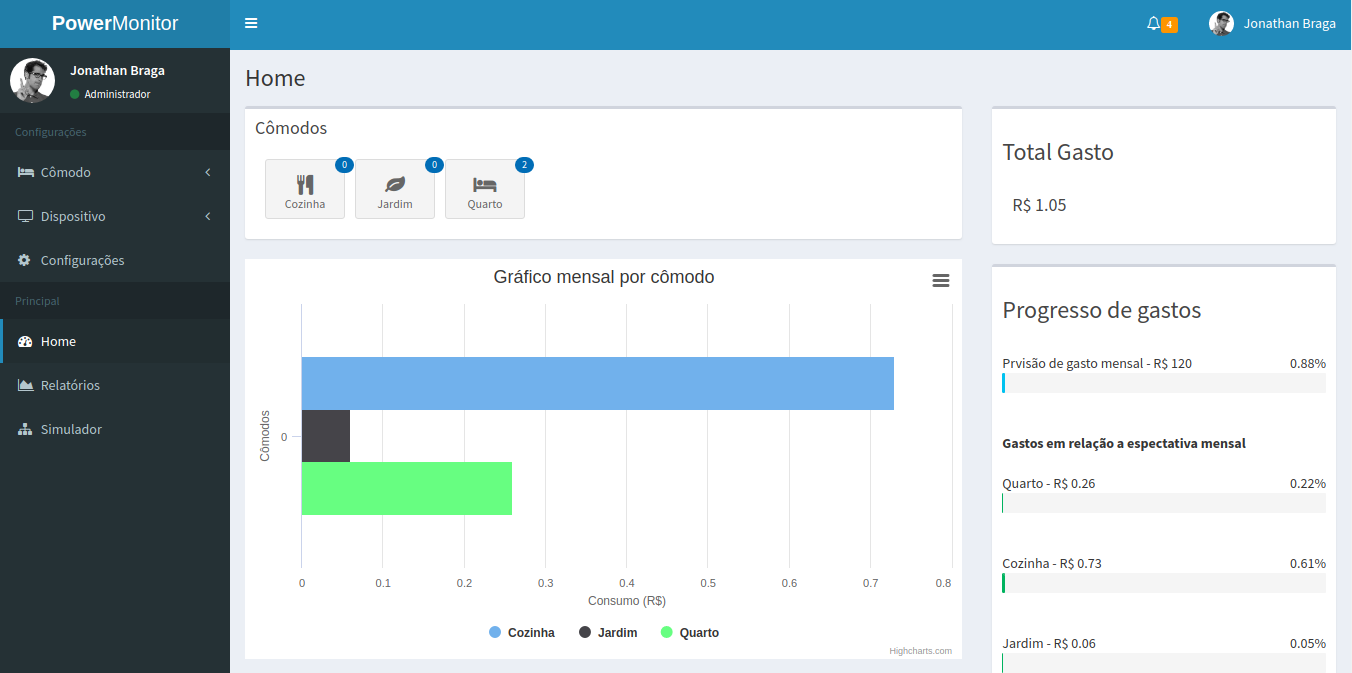
\includegraphics[width=1.0\textwidth, keepaspectratio=true]{principal}
	\centering
	\caption[Tela inicial do sistema]{Tela inicial do sistema}
	\label{fig:principal-ft}
\end{figure}
\FloatBarrier

Todas as informações colhidas pelo servidor \textit{web} em \textit{node.js} (\autoref{node}), são recebidas e tratadas pelo sistema \textit{web}. Os dados
são importantíssimos, pois mediante eles é que se torna possível a contrução dos gráficos e das previsões fornecidas pelo sistema. No \textit{power monitor}
a forma de comunicação com o banco de dados é feita mediante as chamadas de API, existe uma chamada para cada ação prevista no sistema. A \autoref{fig:api-ft}
retrata bem esse cenário, pode-se perceber que o \textit{end-point} (expressão utilizada para se referenciar a uma extremidade de um canal de comunicação.) 
\textbf{get-comodos} é destinado a obtenção de todos os cômodos cadastrados já o \textit{end-point} \textbf{get-dispositivos} é destinado a 
obtenção de todos os dispostivos cadastrados. O motivo da comunicação entre servidor \textit{web} e sistema \textit{web}
ser feita via chamada de API é bem simples, pois qualquer sistema seja \textit{web, desktop} ou qualquer outro tipo, basicamente precisa ter uma comunicação com uma rede \textit{Wi-Fi}
para utilizar o \textit{power monitor}. O \textit{software web} não precisa obrigatoriamente de internet para poder funcionar, pois a comunicação entre servidor e sistema é
baseada em uma rede local, justamente para que o \textit{software} não dependa de terceiros. Para uma perfeita comunicação o ambiente só precisa está configurado
na mesma rede \textit{Wi-Fi}. 

\begin{figure}[h!]
	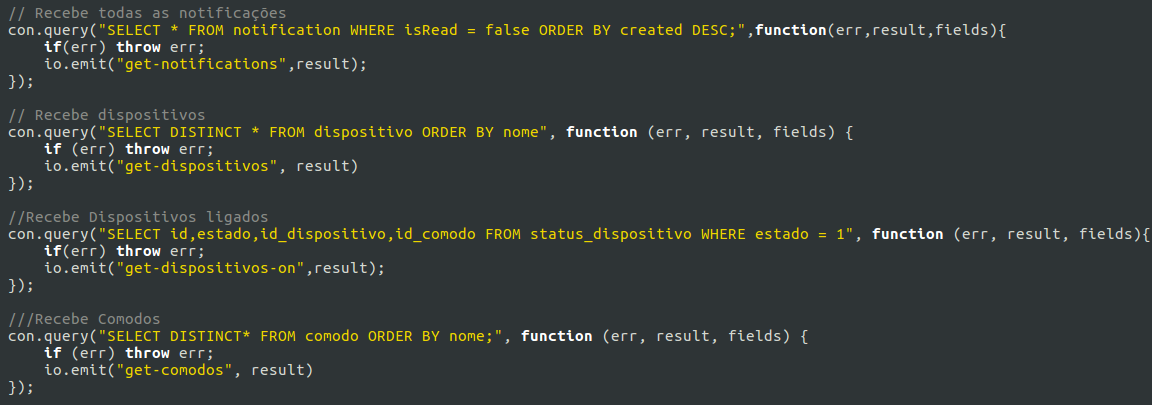
\includegraphics[width=1.0\textwidth, keepaspectratio=true]{api}
	\centering
	\caption[Chamada de API]{Chamada de API}
	\label{fig:api-ft}
\end{figure}
\FloatBarrier

O \textit{software} pode ser dividido em duas partes, servidor \textit{web} e interface \textit{web}. O servidor foi desenvolvido usando a linguagem
\textit{javascript} (\autoref{js}) e para auxílio foi utilizado o \textit{framework node.js} (\autoref{node}), a comunicação entre servidor e banco de dados
é feita pelo \textit{MySQL Server} (\autoref{sql}). A interface \textit{web} é o agente consumidor de todos esses serviços, com uma comunicação via 
\textit{webscoket} (\autoref{websocket}) com o servidor é capaz de receber e enviar dados a qualquer instante. A combinação desses três serviços - servidor \textit{web},
servidor do banco de dados e interface \textit{web} - resultou em uma aplicação intuitiva e amigável, desenvolvida para dar o total suporte às análises do dados
enviados pelo \textit{hardware}. A \autoref{fig:banco-dados} representa o esquema das tabelas do banco de dados que foi utulizado no \textit{power monitor}.

Como já foi apresentada a \autoref{fig:principal-ft} representa a tela inicial da interface \textit{web}, vê-se que é possível
visualizar o total gasto no mês atual, o progresso dos gastos por cômodo que por sua vez é baseado na espectativa de gasto mensal (\autoref{fig:configuracao-ft}), a lista
de todos os cômodos cadastrados e um gráfico mostrando o consumo por cômodo referente ao mês atual.

\begin{figure}[h!]
	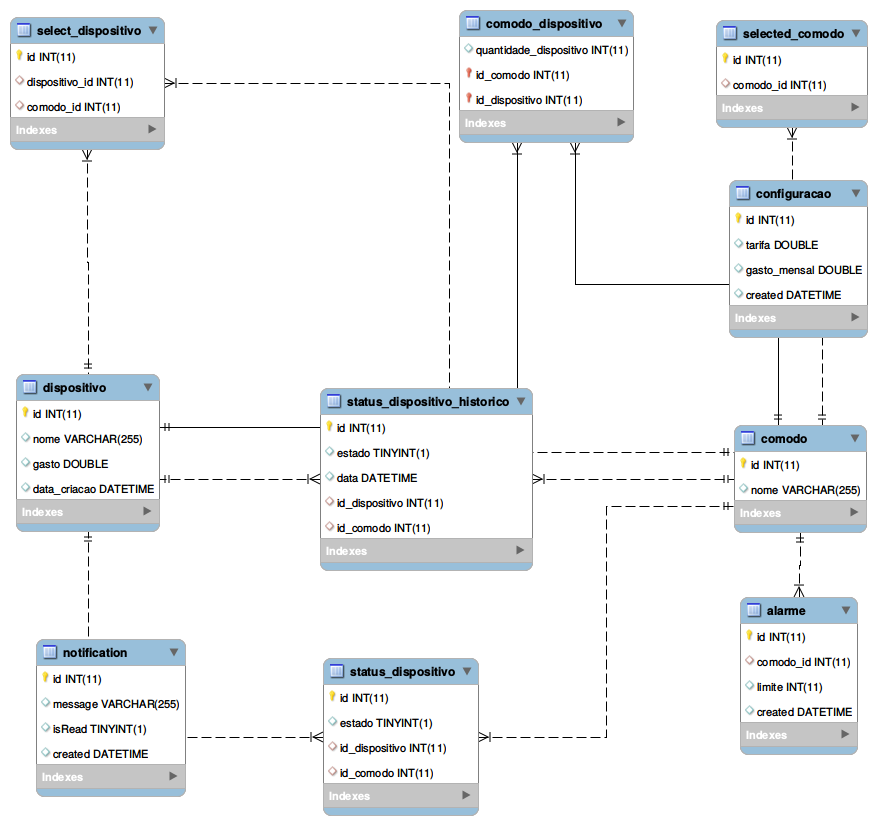
\includegraphics[width=1.0\textwidth, keepaspectratio=true]{banco}
	\centering
	\caption[Esquema das tabelas do banco de dados]{Esquema das tabelas do banco de dados}
	\label{fig:banco-dados}
\end{figure}
\FloatBarrier

As figuras: \ref{fig:c-comodo}, \ref{fig:l-comodo}, \ref{fig:c-dispositivo}, \ref{fig:l-dispositivo} e \ref{fig:configuracao-ft}, 
são relacionadas as telas de cadastro, listagem e de configuração da interface \textit{web}. Nelas é possível cadastrar e listar comodôs e dispositivos assim como 
configurar alguns parâmetros do sistema como o preço da trarifa cobrado por quilowatt-hora pela empresa resposável e a espectativa de gasto mensal.

Uma vez que os cômodos, dispositivos e parâmetros são cadastrados no sistema é possível gerencia-los através da edição ou exclusão dos dados, que se torna possível
nas telas de listagem, para os cômodos e dispositivos, já os parâmetros do sistema na própria tela de configuração se faz a edição dos dados. 

\begin{figure}[h!]
	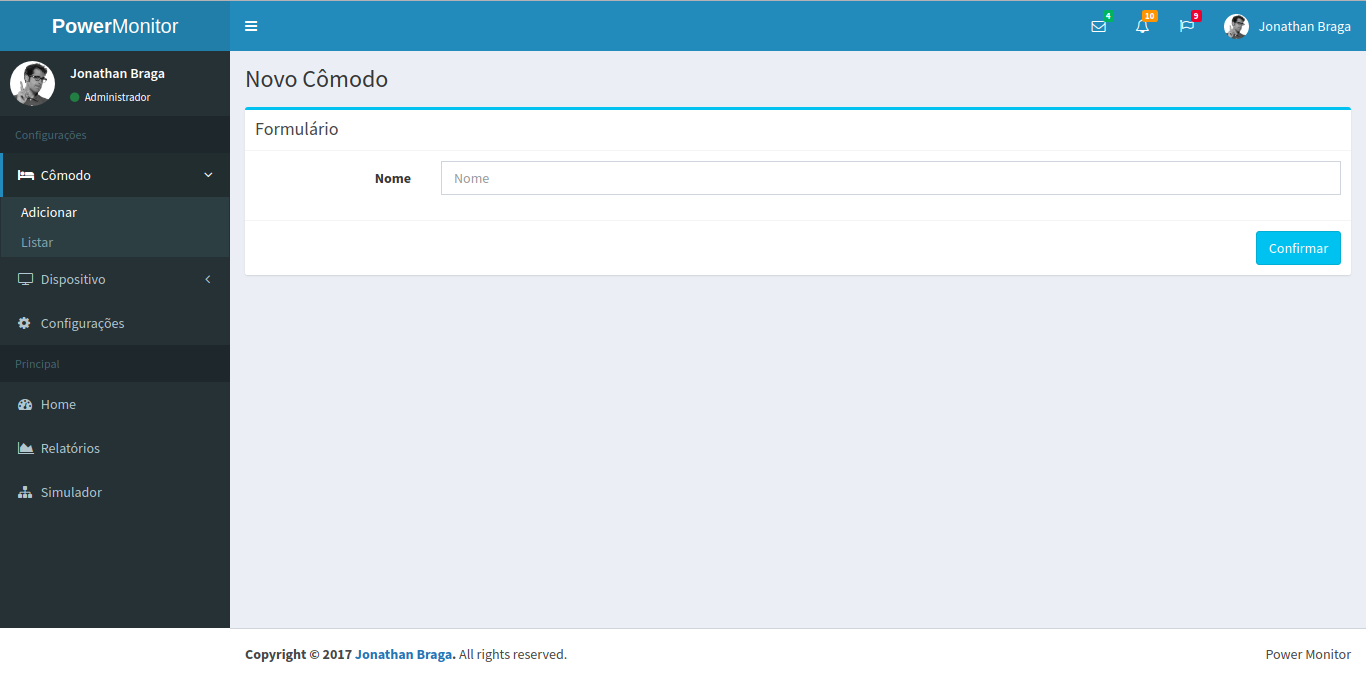
\includegraphics[width=1.0\textwidth, keepaspectratio=true]{c-comodo}
	\centering
	\caption[Cadastro de um cômodo]{Cadastro de um cômodo}
	\label{fig:c-comodo}
\end{figure}
\FloatBarrier

\begin{figure}[h!]
	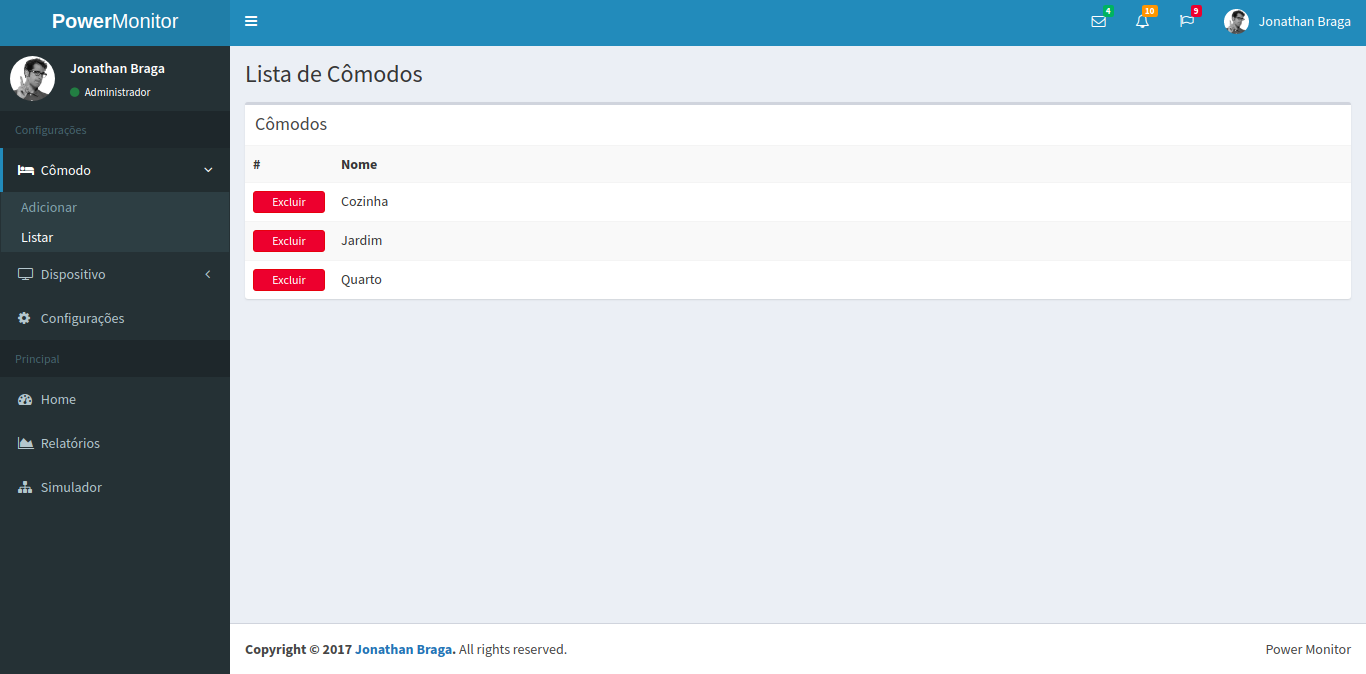
\includegraphics[width=1.0\textwidth, keepaspectratio=true]{l-comodo}
	\centering
	\caption[Lista dos cômodos cadastrados]{Lista dos cômodos cadastrados}
	\label{fig:l-comodo}
\end{figure}
\FloatBarrier

\begin{figure}[h!]
	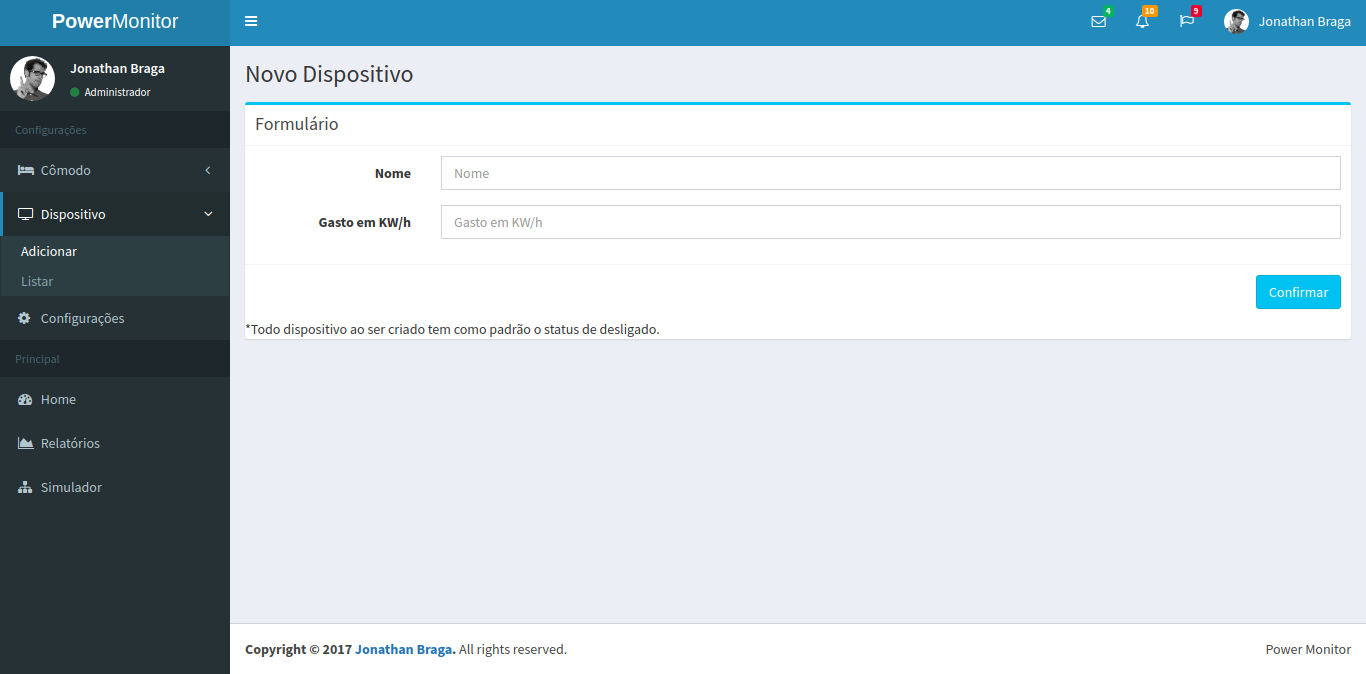
\includegraphics[width=1.0\textwidth, keepaspectratio=true]{c-dispositivo}
	\centering
	\caption[Cadastro de um dispositivo]{Cadastro de um dispositvio}
	\label{fig:c-dispositivo} 
\end{figure}
\FloatBarrier

\begin{figure}[h!]
	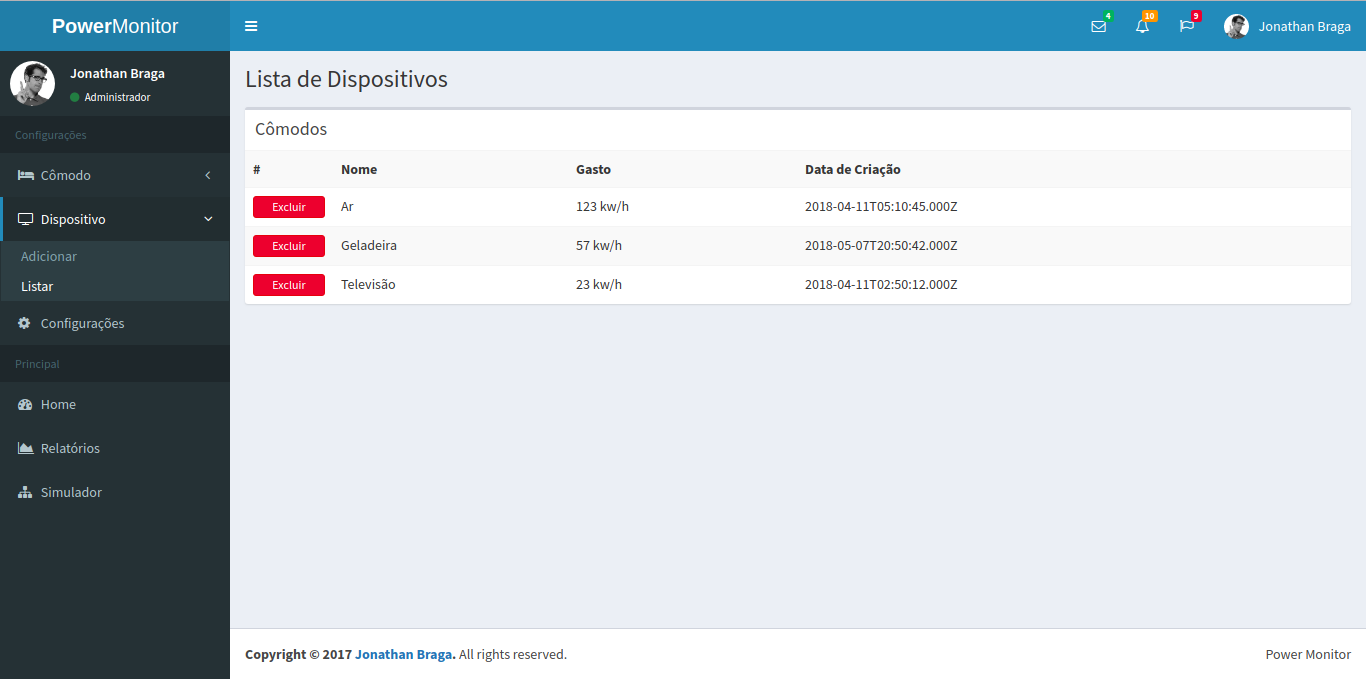
\includegraphics[width=1.0\textwidth, keepaspectratio=true]{l-dispositivo}
	\centering
	\caption[Listagem dos dispositivos cadastrados]{Listagem dos dispositivos cadastrados}
	\label{fig:l-dispositivo} 
\end{figure}
\FloatBarrier

\begin{figure}[h!]
	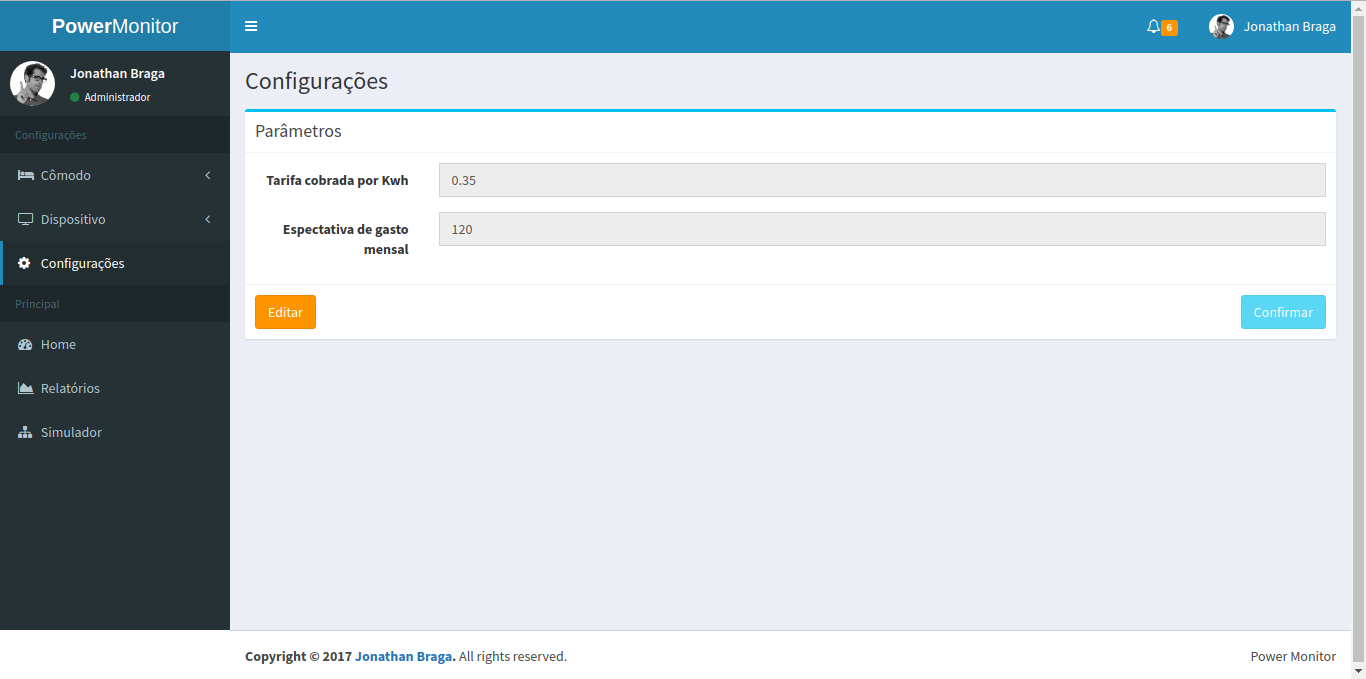
\includegraphics[width=1.0\textwidth, keepaspectratio=true]{configuracao}
	\centering
	\caption[Tela de configuração dos parâmetros do sistema]{Tela de configuração dos parâmetros do sistema}
	\label{fig:configuracao-ft} 
\end{figure}
\FloatBarrier

Uma vez que todos os cômodos, dispositivos e parâmetros já se encontram cadastrados e já exista a comunicação establecida com o hardware, a interface
\textit{web} disponibiliza um séria de formas para visualização das informações coletadas e tratadas. Na \autoref{fig:extrato} é possível visualizar
uma espécie de extrato do consumo de todos os dispositivos, podendo perceber quando foram ligados, quando foram desligados e assim resultando no total gasto.
Já as figuras: \ref{fig:ano-c}, \ref{fig:matu-c} e \ref{fig:mant-c} referem-se aos gráficos que são contruídos baseados nas informações coletadas pelo sistema.

Os gráficos por sua vez são construídos mediante aos calculos que o sistema faz usando como base a \autoref{eq-consumo}, o resusltado dessa conta
fornece ao sistema o consumo em reais (R\$) do dispostivo em um dado intervalo de tempo conhecido. Vale salientar que o resultado é o esperado já que o consumo
do dispositivo (KWh) é pré definido pelo usuário (\autoref{fig:c-dispositivo}), para o cálculo real do consumo usa-se a \autoref{eq-potencia} que leva em conta a corrente real que passa
pelo dispositivo ao longo do tempo que ele permanece ligado. Com esses dados é que se torna possível a construção dos gráficos e extrado presentes no sistema.

\begin{equation} \label{eq-consumo}
	\frac{consumo \, \, do \, \, dispositivo \times tempo \, \, de \, \, uso}{número \, \, de \, \, dias \, \, no \, \, mês} \times tarifa
\end{equation}

\begin{equation} \label{eq-potencia}
	 \frac{ (tensão \times corrente) \times horas \, \, de \, \, uso \, \, por dia \times número \, \, de \, \, dias \, \, no \, \, mês}{1000}
\end{equation} 

\begin{figure}[h!]
	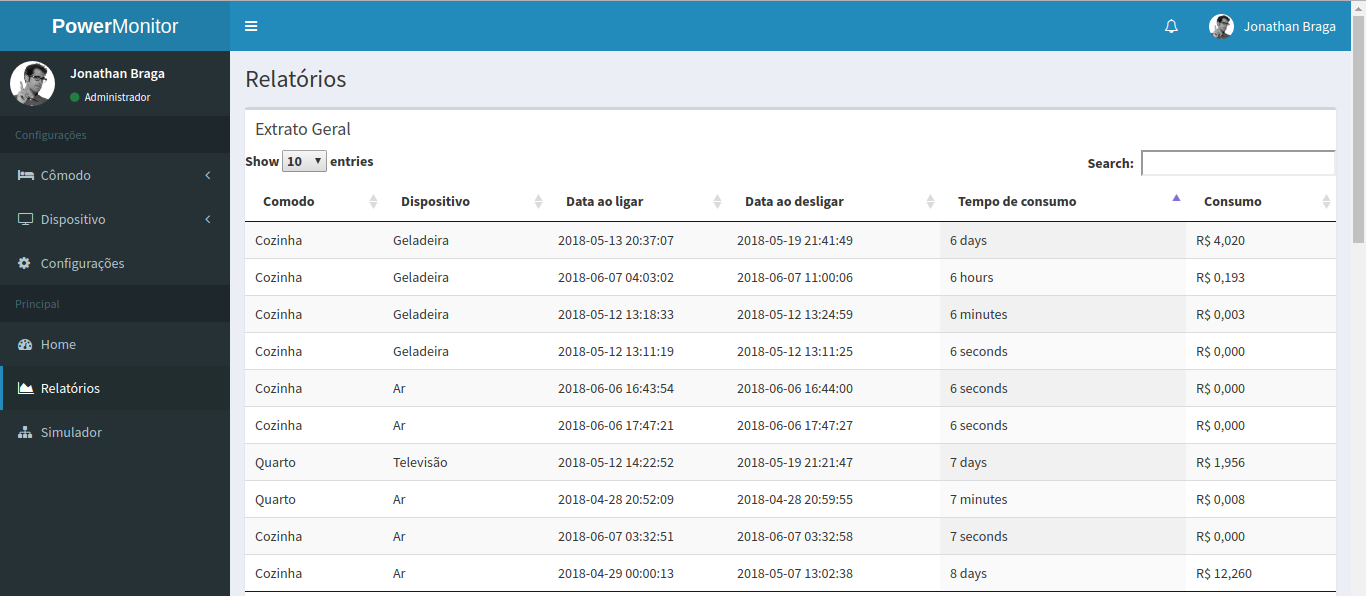
\includegraphics[width=1.0\textwidth, keepaspectratio=true]{extrato}
	\centering
	\caption[Demonstrativo do gasto de cada dispositivo]{Demonstrativo do gasto de cada dispositivo}
	\label{fig:extrato} 
\end{figure}
\FloatBarrier

\begin{figure}[h!]
	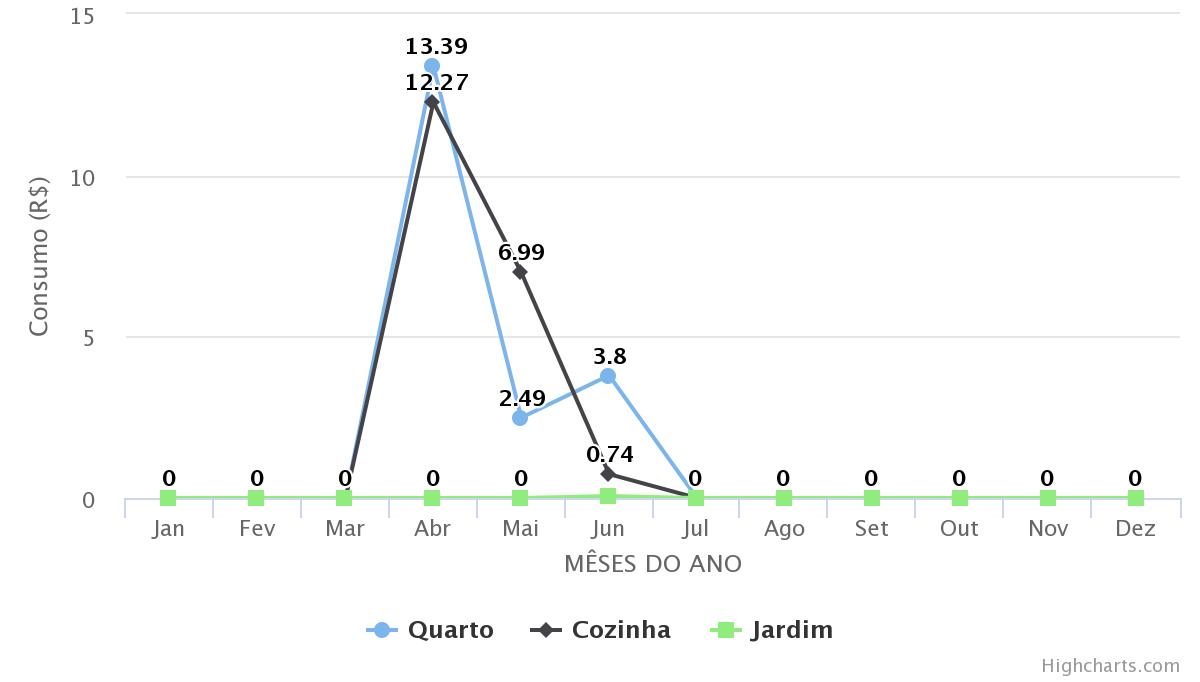
\includegraphics[width=1.0\textwidth, keepaspectratio=true]{ano-c}
	\centering
	\caption[Consumo geral de todos os dispositivos por cômodo ao longo do ano]{Consumo geral de todos os dispositivos por cômodo ao longo do ano}
	\label{fig:ano-c} 
\end{figure}
\FloatBarrier

\begin{figure}[h!]
	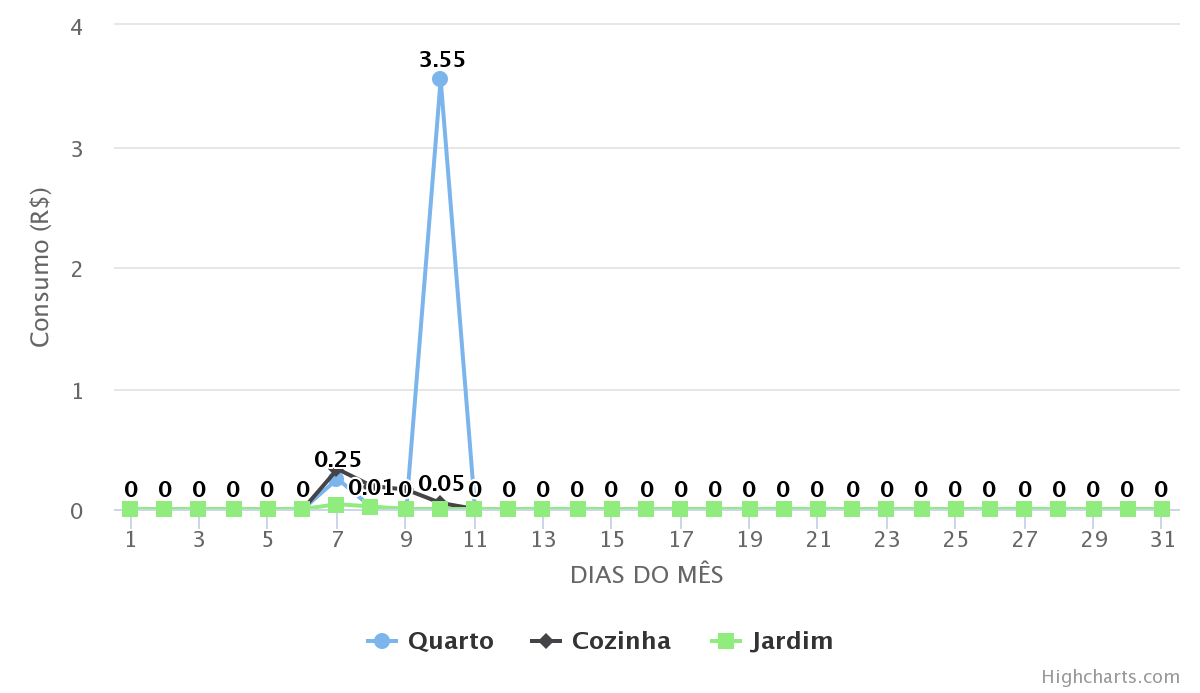
\includegraphics[width=1.0\textwidth, keepaspectratio=true]{matu-c}
	\centering
	\caption[Consumo geral de todos os dispositivos por cômodo ao longo do mês atual]{Consumo geral de todos os dispositivos por cômodo ao longo do mês atual}
	\label{fig:matu-c} 
\end{figure}
\FloatBarrier

\begin{figure}[h!]
	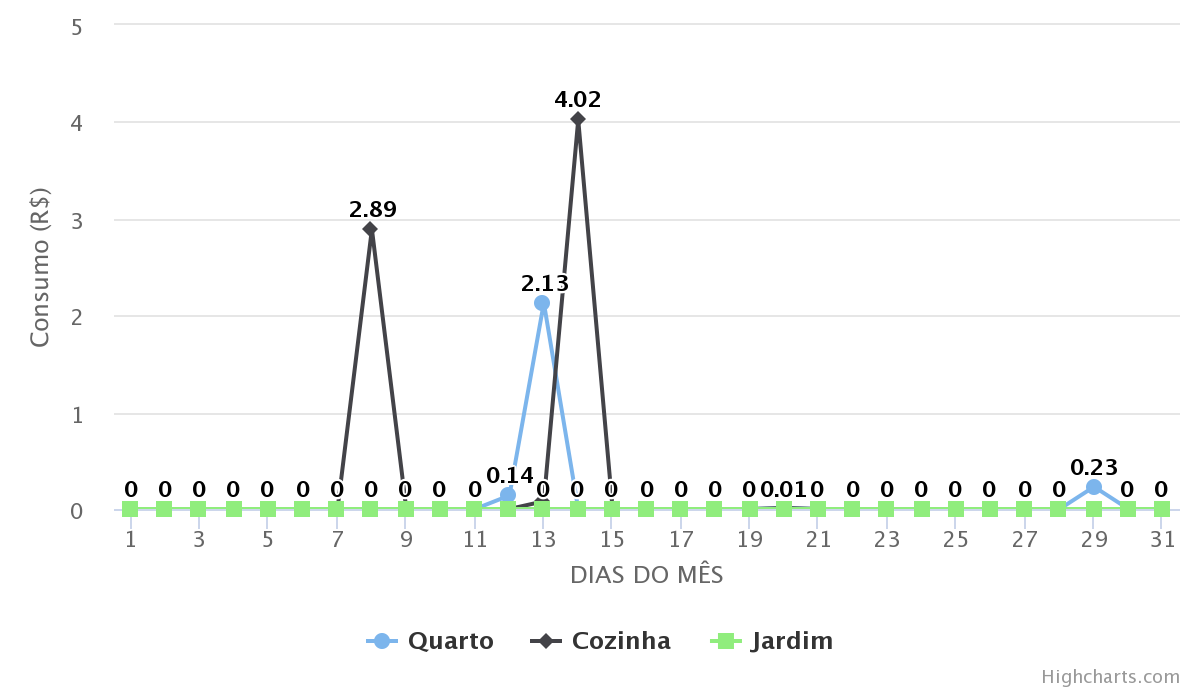
\includegraphics[width=1.0\textwidth, keepaspectratio=true]{mant-c}
	\centering
	\caption[Consumo geral de todos os dispositivos por cômodo ao longo do mês anterior]{Consumo geral de todos os dispositivos por cômodo ao longo do mês anterior}
	\label{fig:mant-c} 
\end{figure}
\FloatBarrier

O \textit{softaware} também possui um local específico para a gerência dos cômodos, um espaço destinado para a vinculação de dispositivos ao cômodo,
visualização do total gasto em relação ao mês atual em forma de gráfico e a opção de ligar, desligar ou excluir o dispostivo do cômodo. As figuras:
\ref{fig:comodo-ft}, \ref{fig:v-dispositivo} e \ref{fig:a-dispositivo} retratam o cenário descrito.

\begin{figure}[h!]
	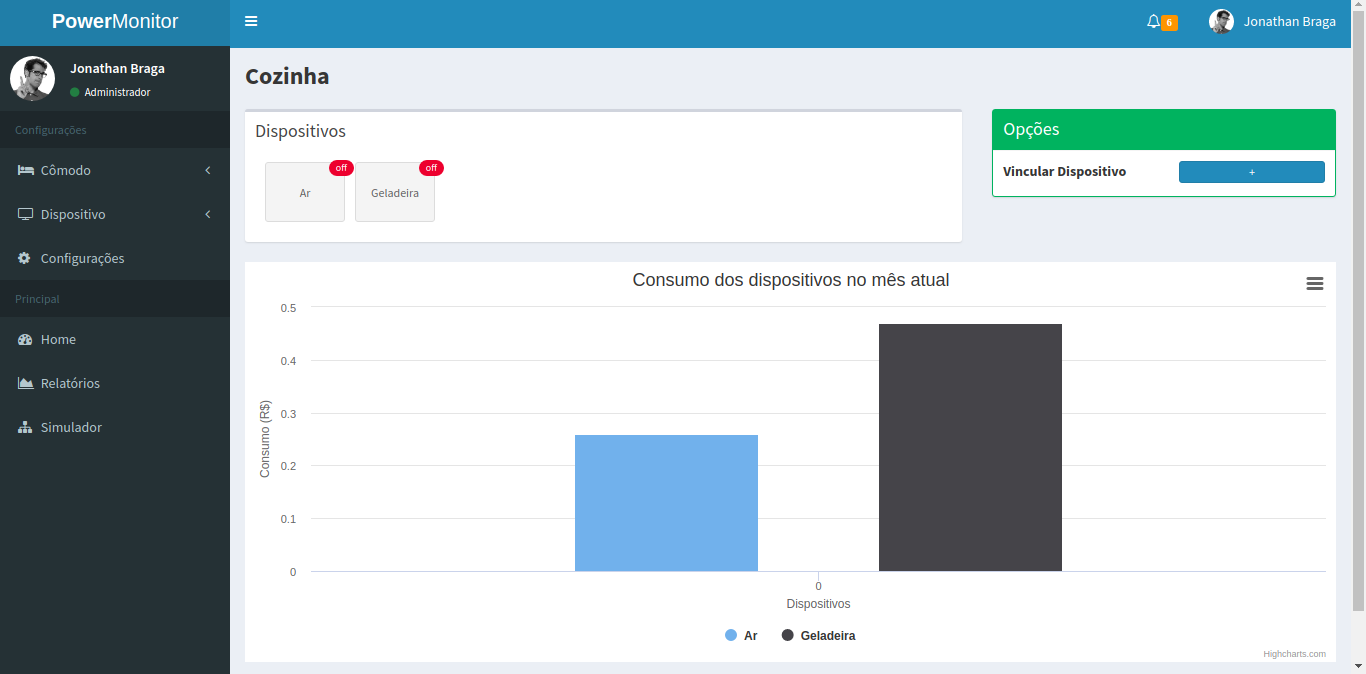
\includegraphics[width=1.0\textwidth, keepaspectratio=true]{comodo}
	\centering
	\caption[Visão geral da gerência de um cômodo]{Visão geral da gerência de um cômodo}
	\label{fig:comodo-ft} 
\end{figure}
\FloatBarrier

\begin{figure}[h!]
	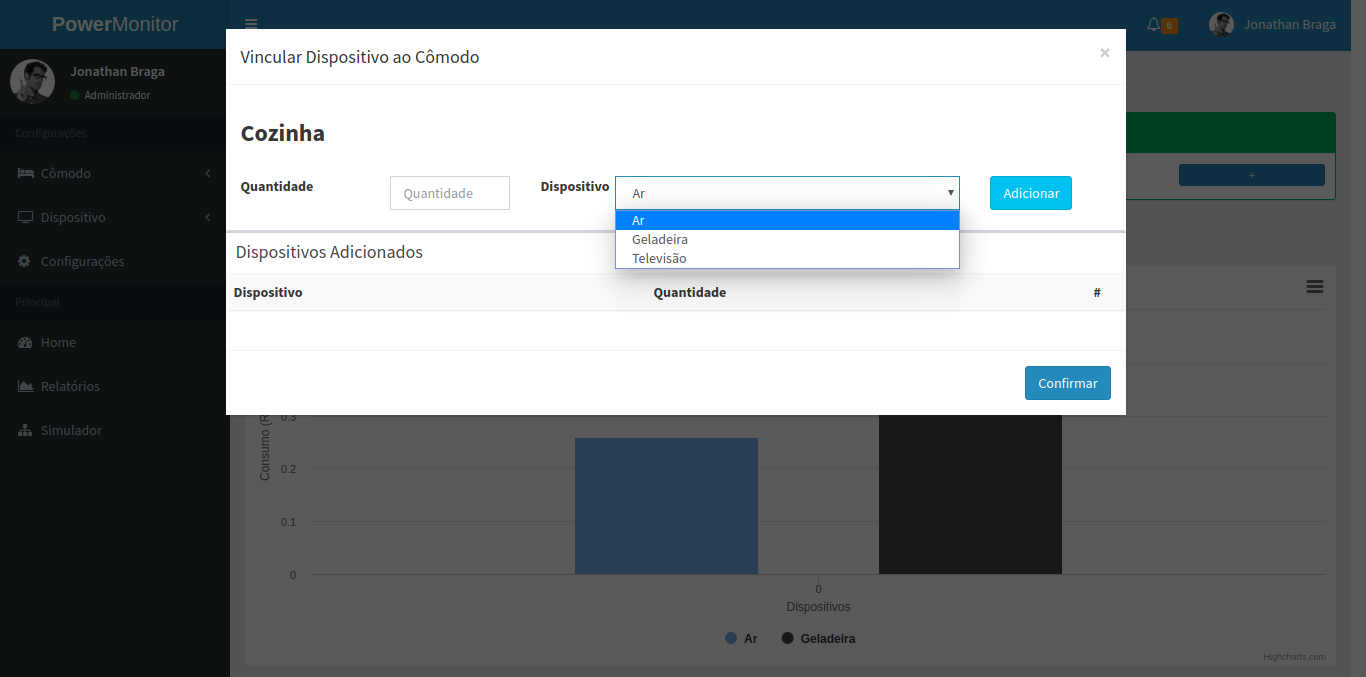
\includegraphics[width=1.0\textwidth, keepaspectratio=true]{v-dispositivo}
	\centering
	\caption[Vincular dispositivo ao cômodo]{Vincular dispositivo ao cômodo}
	\label{fig:v-dispositivo} 
\end{figure}
\FloatBarrier

\begin{figure}[h!]
	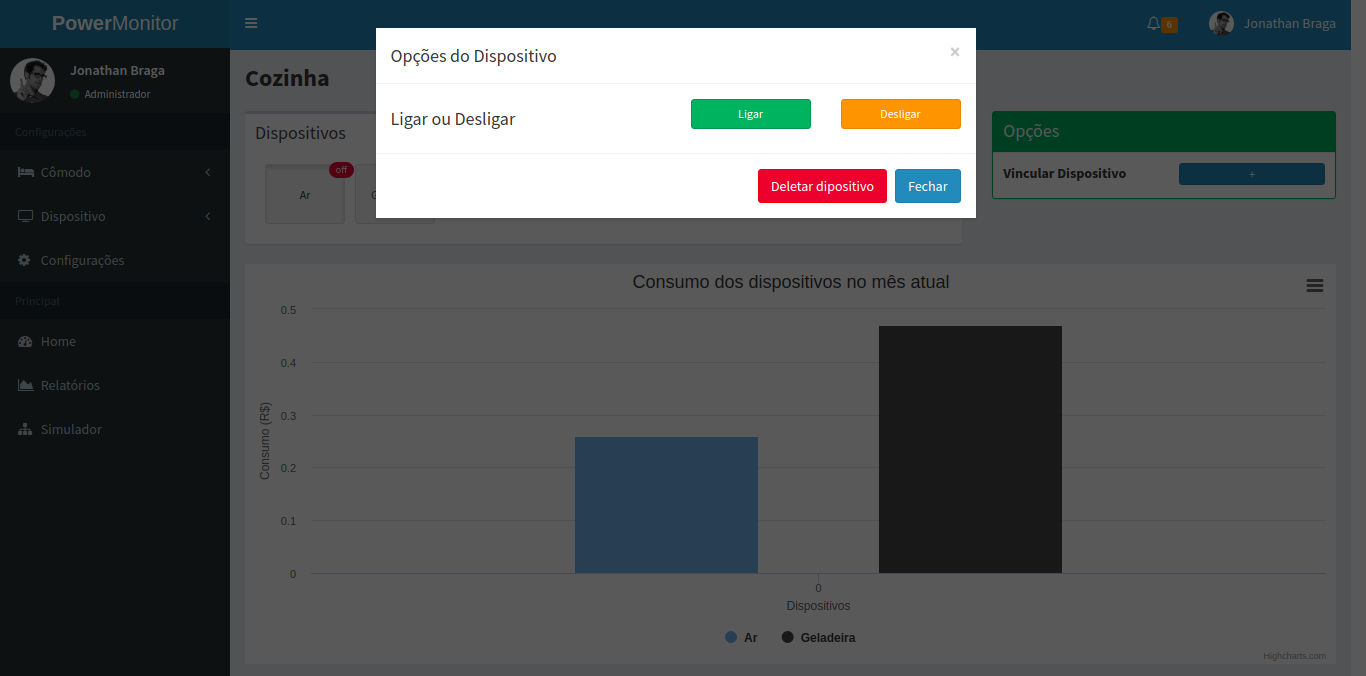
\includegraphics[width=1.0\textwidth, keepaspectratio=true]{a-dispositivo}
	\centering
	\caption[Ações que podem ser realizadas no dispositivo vinculado]{Ações que podem ser realizadas no dispositivo vinculado}
	\label{fig:a-dispositivo} 
\end{figure}
\FloatBarrier

Outras duas funcionalidades presentes no sistema são os alarmes gerados quando o usuário passa dos 50\% e dos 80\% do consumo esperado, cadastrado previamente pelo mesmo.
Também existe um simulador de gastos, onde é possível calcular o gasto mensal e diário que um dispositivo irá trazer para uma residência. As figuras
\ref{fig:aviso-a}, \ref{fig:aviso-v} e \ref{fig:simulador} retratam o descrito.

\begin{figure}[h!]
	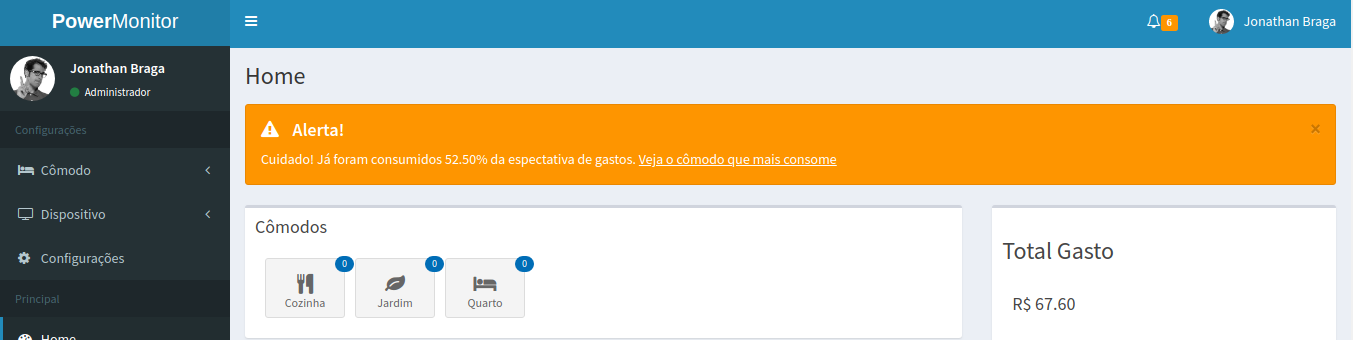
\includegraphics[width=1.0\textwidth, keepaspectratio=true]{aviso-a}
	\centering
	\caption[Alerta exibido quando o consumo supera os 50\% do previsto]{Alerta exibido quando o consumo supera os 50\% do previsto}
	\label{fig:aviso-a} 
\end{figure}
\FloatBarrier

\begin{figure}[h!]
	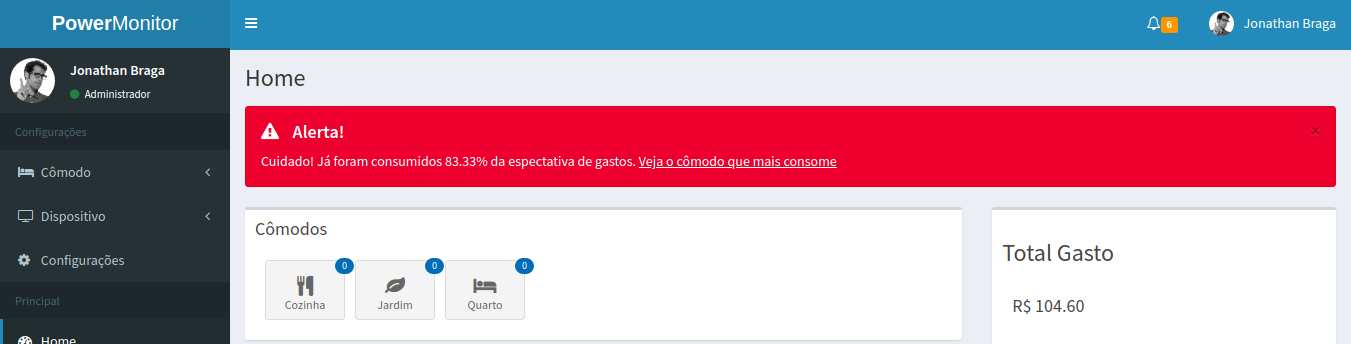
\includegraphics[width=1.0\textwidth, keepaspectratio=true]{aviso-v}
	\centering
	\caption[Alerta exibido quando o consumo supera os 80\% do previsto]{Alerta exibido quando o consumo supera os 80\% do previsto}
	\label{fig:aviso-v} 
\end{figure}
\FloatBarrier

\begin{figure}[h!]
	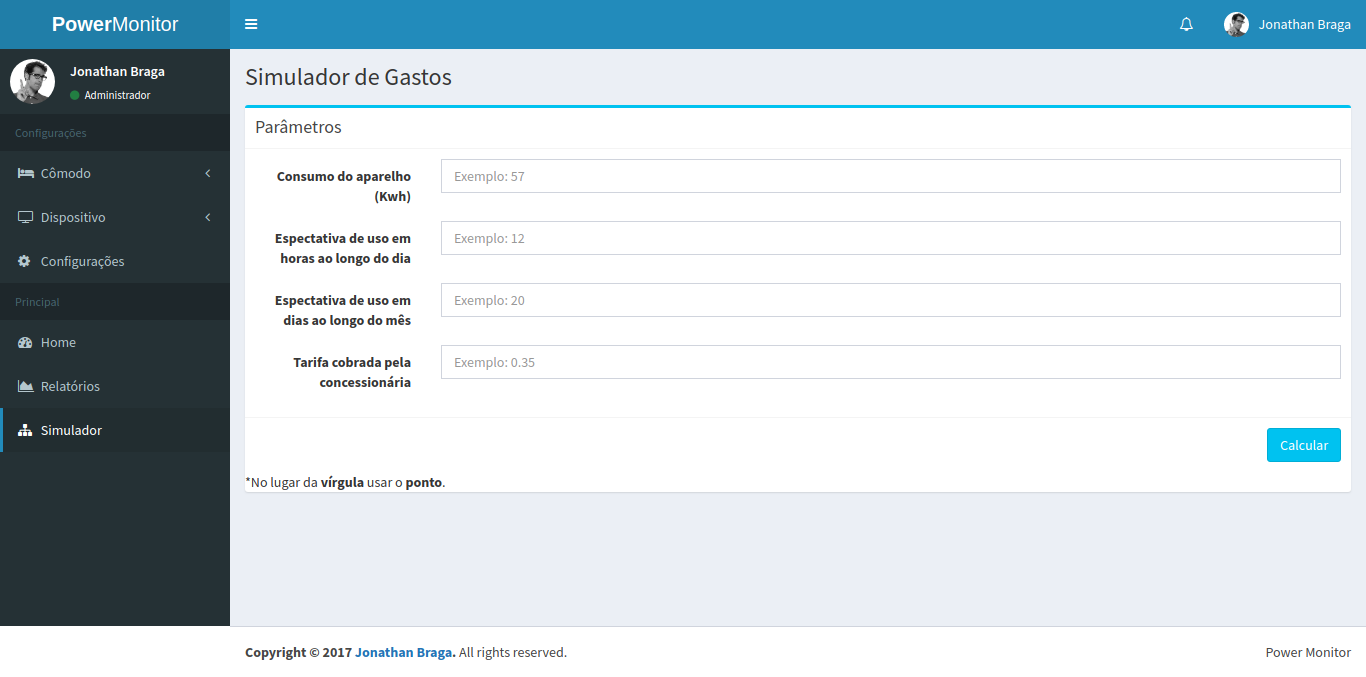
\includegraphics[width=1.0\textwidth, keepaspectratio=true]{simulador}
	\centering
	\caption[Simulador de gastos]{Simulador de gastos}
	\label{fig:simulador} 
\end{figure}
\FloatBarrier

\section[\textit{Hardware}]{\textit{Hardware}}\label{hard-sec}
O desenvolvimento do \textit{hardware} para demonstação da comunicação com o \textit{power monitor} envolve uma série de sensores e componentes
eletrônicos. A plataforma de prototipagem eletrônica utilizada para a construção desse \textit{hardware}, foi o ESP8266(\autoref{esp}). O principal sensor
utilizado foi o SCT 013-000 (\autoref{sct}), que tem o papel de aferir dados da corrente que passa pelos dispositivos ao longo do tempo que o mesmo se encontra
ligado, também vale destacar o uso do relé que é responsável por toda a lógica de liga e desliga do dispositivo. O ESP8266 faz o intermédio da comunicação entre 
\textit{hardware} e servidor \textit{web}, fazendo toda a comunicação eletrônica entre o sensor e o circuito montado (\autoref{fig:circuito}), e enviando os dados
recebidos pelo sensor de corrente para o servidor \textit{web} que por sua vez, salva as medições aferidas no banco de dados. Com relação aos dados enviados 
para o banco, foi feito um algoritmo que ao identificar que o dispositivo está ligado verificando a corrente elétrica no presente momento e quando o mesmo é desligado 
é aferido novamente a corrente elétrica, esse resultado é multiplicado pelo valor da tensão
e assim é obtido o consumo do dispositivo (KWh). Após esse processo a informação é enviada via \textit{webscoket} 
para o servidor \textit{web} que salva tudo no banco de dados, e por fim a informação é consumida pela interface \textit{web}.

É válido lembrar que, para a comunicação \textit{websocket} é necessário o \textit{hardware} e o \textit{softaware} estarem conectados
na mesma rede \textit{Wi-Fi}. O grande motivo para a escolha do ESP8266 como plataforma de prototipagem foi a sua fácil comunicação com uma rede
\textit{Wi-Fi}, o código a seguir é um exemplo de como estabelecer a comunicação com uma rede sem fio.

\newpage

\begin{lstlisting}
	#include <ESP8266WiFi.h>
	const char* ssid = NOME DA REDE;
	const char* password = SENHA;
	
	WiFi.begin(ssid, password);
\end{lstlisting}

Após estabelecer a conexão o próximo passo será interligar o servidor \textit{web} com o \textit{hardware} através da comunicação por \textit{websocket},
que será facilitada por meio da biblioteca \textit{SocketIOClient}, ela fornece alguns métodos como: \textit{\textbf{emit}}\protect\footnotemark, \textit{\textbf{on}}\protect\footnotemark 
e \textit{\textbf{connect}}\protect\footnotemark  que ajudam no momento de concretizar a comunicação total do \textit{hardware}. A seguir terá um
exemplo de como usar os métodos citados com o código anterior.

\addtocounter{footnote}{-2}
\footnotetext{Função responsável por emitir os dados para o servidor \textit{web}}
\addtocounter{footnote}{1}
\footnotetext{Função responsável por receber os dados do servidor \textit{web}}
\addtocounter{footnote}{1}
\footnotetext{Função responsável por estabelecer conexão com servidor \textit{web}}

\begin{lstlisting}
	#include <SocketIOClient.h>
	SocketIOClient socket;
	const char* ssid = NOME DA REDE;
	const char* password = SENHA;
	String host = IP DO SERVIDOR WEB;
	int port = PORTA QUE FOI FORNECIDA AO SERVIDOR WEB;	

	void led(String state) {
	Serial.println("[led] " + state);
	if (state == "\"state\":true") {
	socket.emit("post-informacao","{\"data\":\"1\"}");
	}
	else {
	socket.emit("post-informacao","{\"data\":\"0\"}");
	}
	}

	void setup() {
		WiFi.begin(ssid, password);
  		socket.on("ligar", ligar);  
  		socket.connect(host, port);
	}

	void loop() {
  		socket.monitor();    
	}
\end{lstlisting}

A \autoref{fig:circuito} mostra bem o circuito demonstrativo utilizado neste trabalho para exemplificar a comunicacação com o \textit{power monitor}.
O esquema representa uma forma prática e simples de se usar o sensor de corrente, o SCT 013-000 é ativado quando o usuário liga a lâmpada no interruptor
(representado por um botão) ou pelo sistema \textit{web} (\autoref{fig:a-dispositivo}), fazendo com que o relé ative e permita com que o dispositivo 
mude o estado para ligado. Após esse processo o sistema irá medir corrente que passa pelo dispositivo, e ao ser desligado o resultado
do consumo do dispositivo irá ser transmitido via \textit{websocket} para o servidor \textit{web} e se juntará com o resultado do tempo em que o dispositivo permaneceu
ligado para que por fim se possa se ter o consumo e o gasto deferido pelo equipamento. 

\begin{figure}[h!]
	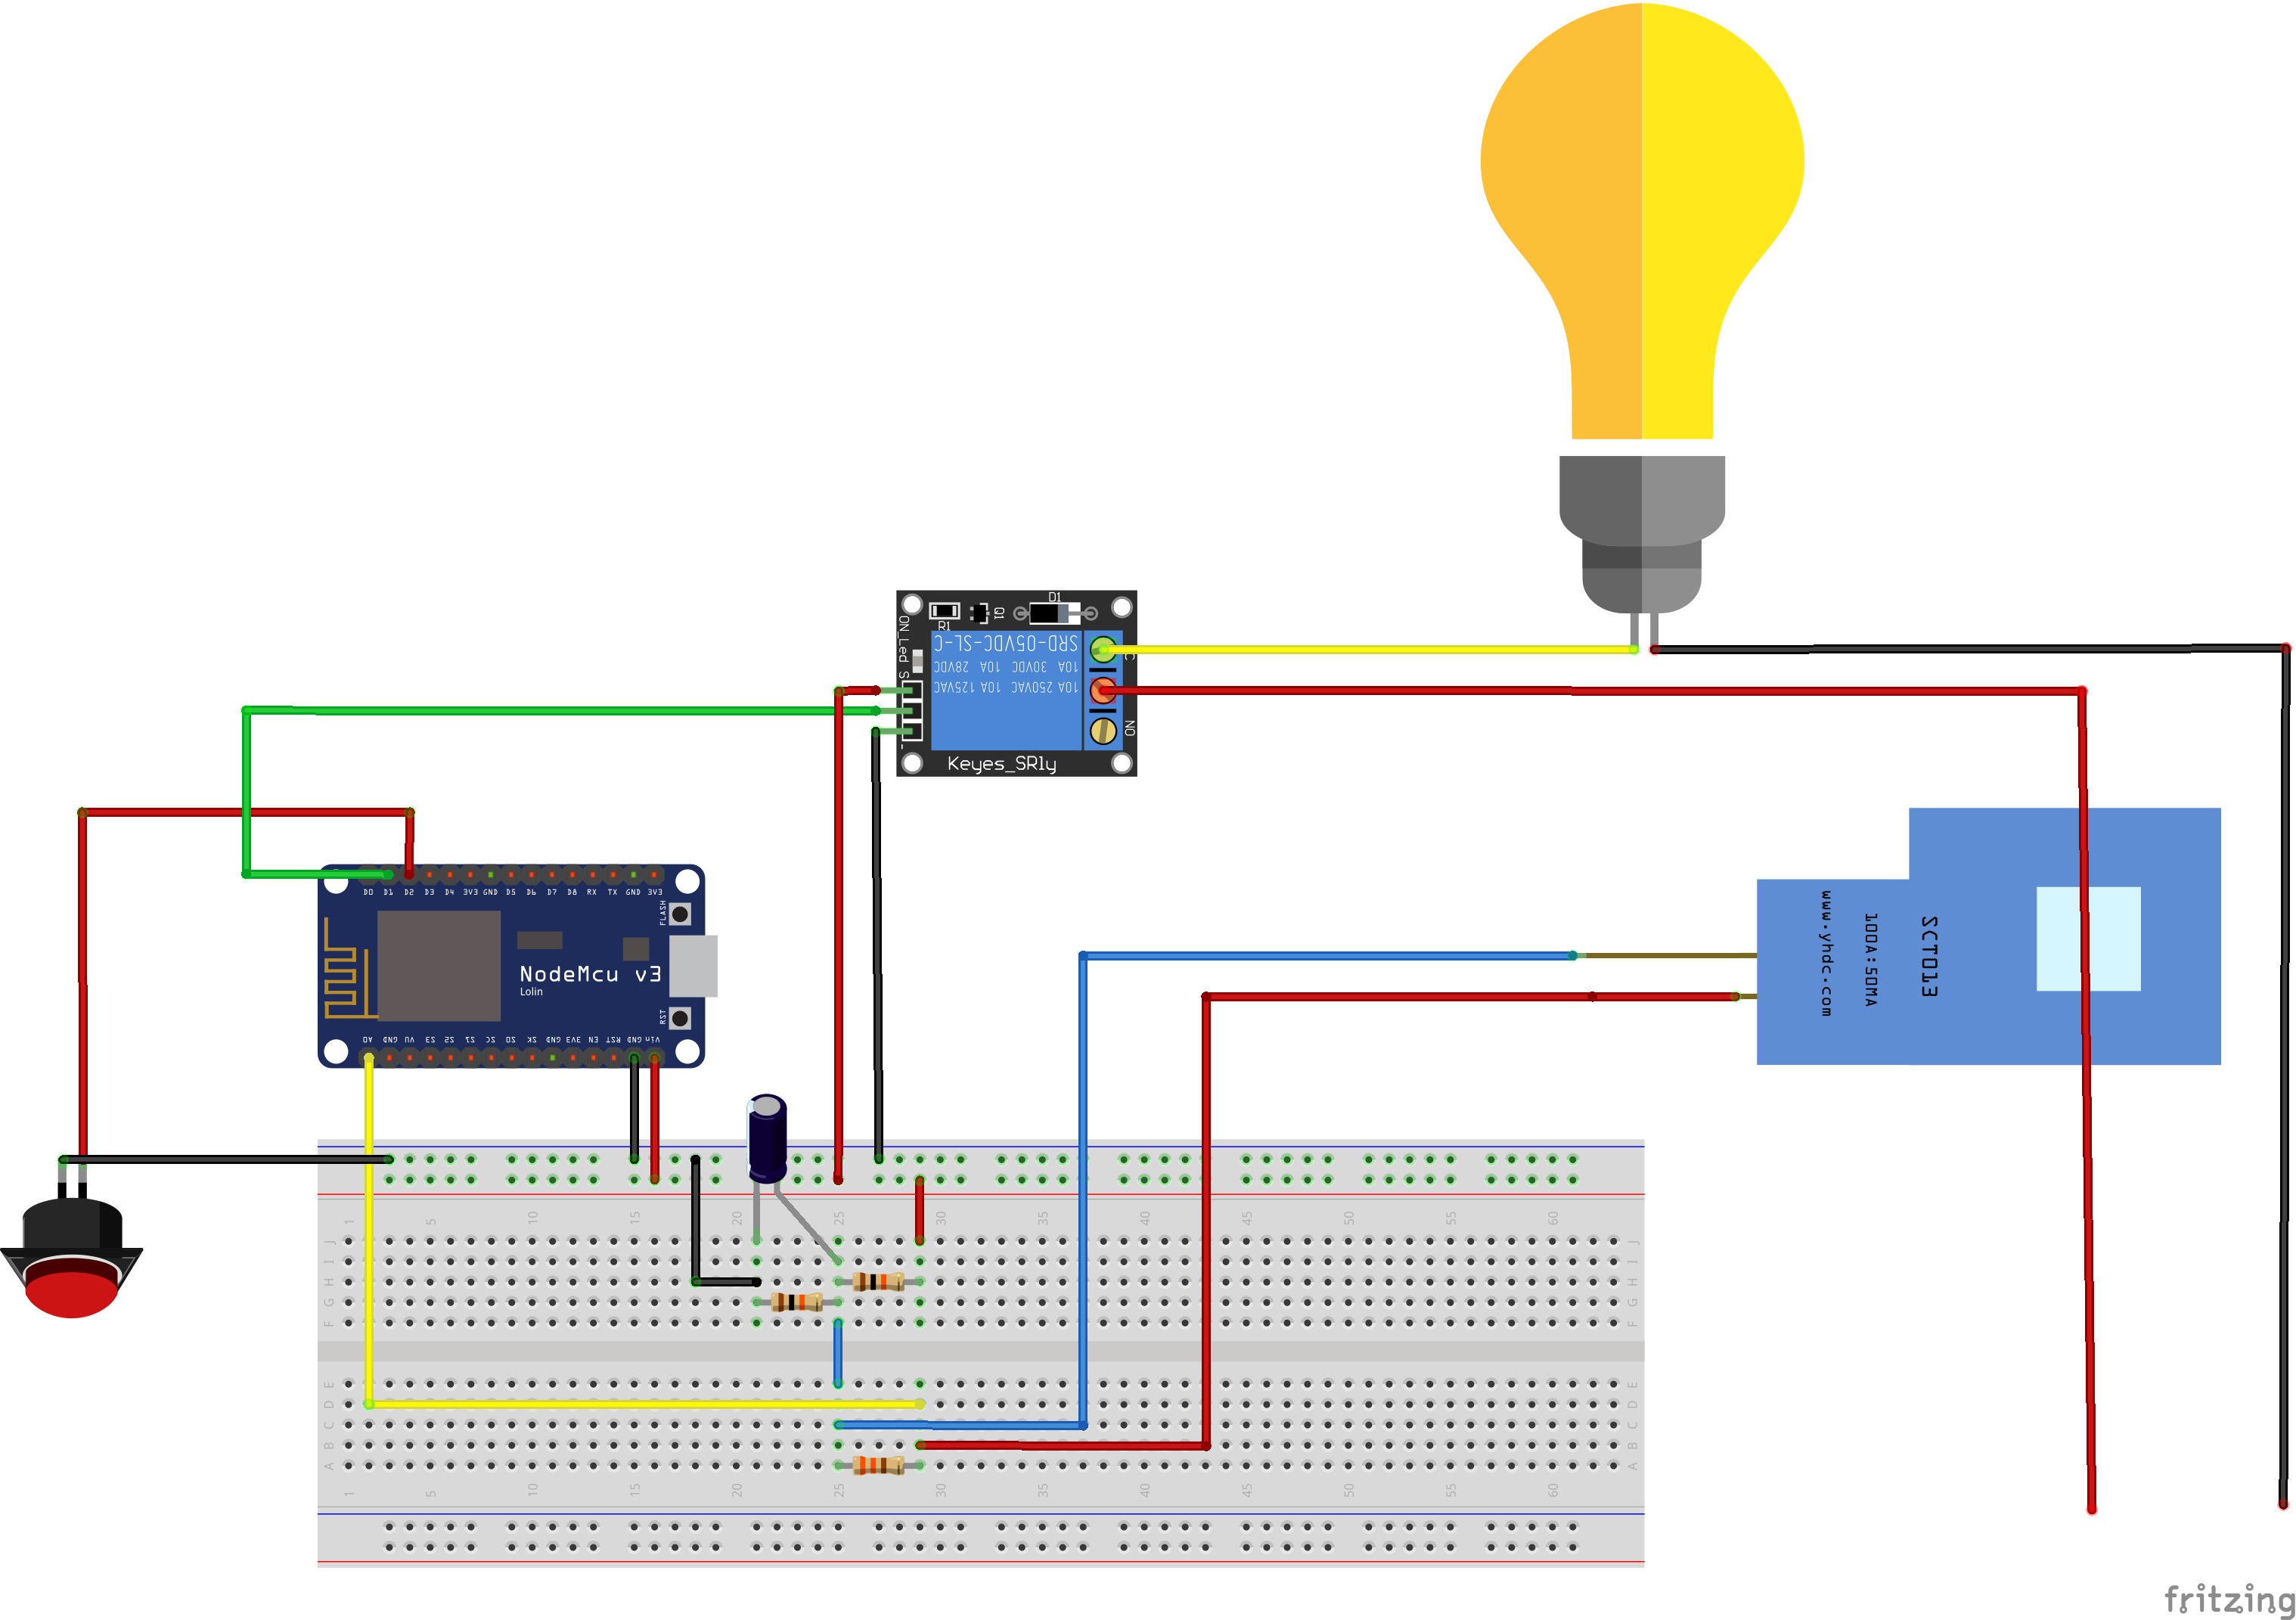
\includegraphics[width=0.8\textwidth, keepaspectratio=true]{circuito}
	\centering
	\caption[Circuito demonstrativo para comunicação com o \textit{power monitor}]{Circuito demonstrativo para comunicação com o \textit{power monitor}}
	\label{fig:circuito}  
\end{figure}
\FloatBarrier

\section[\textit{Resultados}]{\textit{Resultados}}\label{resultados-sec}

Depois de todo o estudo realizado, possibilidades discutidas e desenvolvimento detalhado, chegou-se ao  funcionamento da primeira versão
do \textit{softaware power monitor}. O sistema disponibiliza meios para uma fácil comunicação com qualquer \textit{hardware} de monitoramento
de energia e uma interface que leva o usuário a ter um novo entendimento e uma nova conscientização sobre o gasto energético. Trazendo uma forma menos
complicada de mensuarar a quantidade de energia elétrica utilizada em uma residência, possibilitando também uma boa e simples leitura de quanto tem se gastado.

O \textit{power monitor} foi pensado para ser uma solução simples e barata, onde qualquer pessoa que tenha os devidos conhecimentos possa 
instalar, comunicar com \textit{hardwares} personalizados ou até mesmo modificar o código fonte. Como o \textit{software} foi desenvolvimento 
para que todos possam usar e modificar, todo o código fonte está disponível na plataforma de hospedagem de código fonte chamada 
\textit{GitHub} no seguinte endereço: \url{https://github.com/jonathanbraga/power-monitor}{}. A \autoref{custo-teste} mostra bem os 
custos do dispositivo que foi utilizado para a demonstração da comunicação com o \textit{power monitor}.


\begin{table}[!ht]
	\centering
	\begin{tabular}{ccc}
		\hline
		\textbf{Quantidade} & \textbf{Dispositivo}               & \textbf{Preço (R\$)}                 \\ \hline
		\rowcolor[HTML]{DDDDDD} 
		2                   & Resistor 10k$\Omega$ & 0,99                                 \\
		1                   & Resistor 330$\Omega$ & 0,99                                 \\
		\rowcolor[HTML]{DDDDDD} 
		1                   & Módulo Relé 5v                     & 9,00                                 \\
		1                   & NodeMCU                            & 59,76                                \\
		\rowcolor[HTML]{DDDDDD} 
		1                   & SCT 013-000                        & 58,80                                \\
		1                   & Capacitor eletrolítico 100uF       & 2,47                                 \\
		\rowcolor[HTML]{DDDDDD} 
		1                   & Conjunto de 40 Jumpers             & 9,00                                 \\
		1                   & Protoboard             & 20,00                                 \\
		1                   & Chave gangorra 2 terminais         & 3,00                                 \\ \hline
		\multicolumn{2}{|c|}{\textbf{TOTAL}}                     & \multicolumn{1}{c|}{\textbf{165,00}} \\ \hline
	\end{tabular}
	\caption{Custos do dispositivo de demonstração}
	\label{custo-teste}
\end{table} 

% Capitulo 4
\chapter[Capítulo 4]{Capítulo 4}
\label{ch:cap4}
\lipsum[3-5]

\section{Seção}

\lipsum[1-2]

\subsection{Subseção}
\lipsum[3-5]

\section{Seção 2}\label{secao2}

O SHAPE é a sigla em inglês para \textit{Symbolic Hierarchical Automated Reliability and Performance Evaluator}. Veja a  \autoref{fig:sharpe}.

\begin{figure}[!h]
	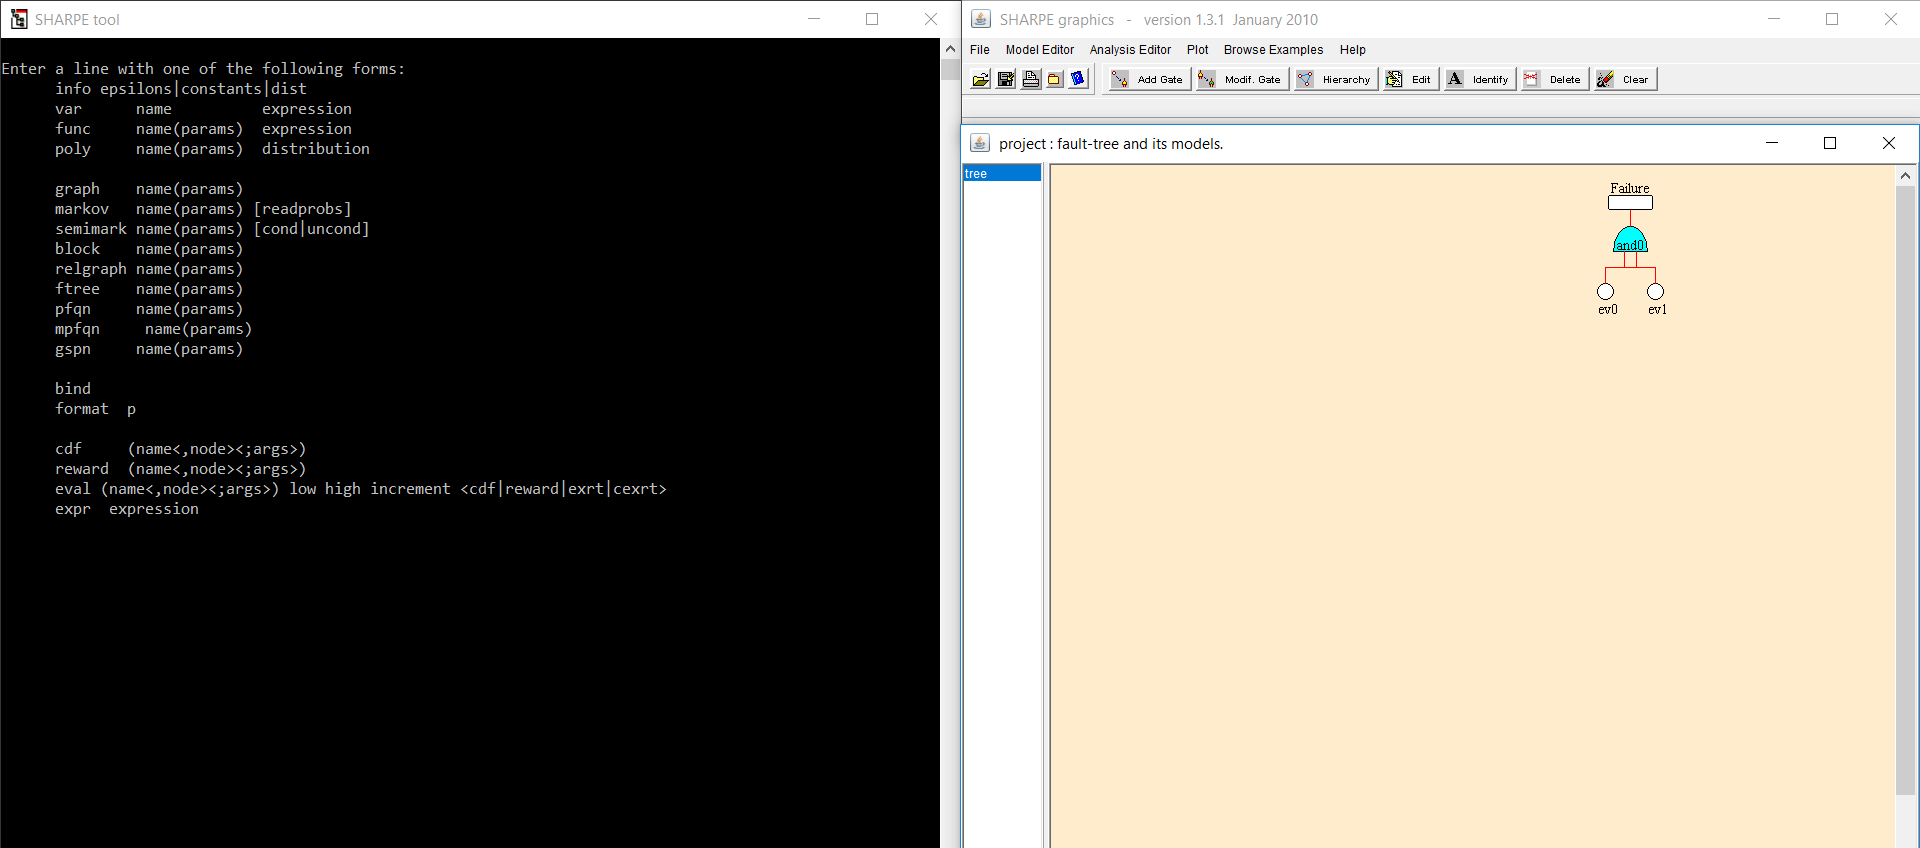
\includegraphics[width=1.0\textwidth, keepaspectratio=true]{sharpe}
	\centering
	\caption[\textit{Print screen} do SHARPE em linha de comando e em interface gráfica.]{\textit{Print screen} do SHARPE em linha de comando e em interface gráfica.}
	\fonte{Elaborada pela autora.}
	\label{fig:sharpe}
\end{figure}

% Capitulo 5
\chapter[Capítulo 5]{Capítulo 5}
\label{ch:cap5}

\lipsum[2-3]

\section{Seção}

\lipsum[3-4]

% Conclusão
\chapter[Conclusão]{Conclusão}
\label{ch:conclusao-cap}

Do início ao fim deste trabalho de conclusão de curso, alguns conceitos foram apresentados
e demonstrados a respeito do consumo de energia elétrica, visando criar um cenário
comparativo a respeito da situação energética do país. Ao longo dos anos o povo brasileiro
ouviu sobre propostas na melhoria do meio ambiente, sustentáveis e até
melhoria na infraestrutura urbana. Porém na maiora das vezes nunca passou de apenas propostas.

Por meio do estudo realizado neste trabalho constatou-se que a leitura do
consumo energético feita em tempo real e disponibilizada para o usuário de uma maneira entendível e direta
desperta a curiosidade e consequentemente a conscientização do mesmo. Apenas mostrar os resultados coletados não seria suficiente
para a conscientização do cidadão brasileiro, a forma com que os resultados são relatados para o consumidor tem um grande impacto, pois
no momento em que a unidade de medida do consumo de energia elétrica é "trocada" do quilowatt-hora para a moeda em circulação no país, o real, 
faz com que todos os brasileiros independente da classe social ou do grau de escolaridade entenda o quanto tem se consumido e disperdiçado em sua residência.

Este trabalho traz uma solução eficiente no monitoramento de energia elétrica, tanto no ambito do \textit{software} como na comunicação com 
\textit{hardware}. O Sistema foi pensado de tal maneira que mesmo em que não exista a presença de um \textit{hardware} para controlar os dispositivos físicos
o utente possa, ainda sim, monitorar os seus gatos por meio das simulações que levam em conta o consumo esperado do dispositivo. A facilidade de estabelecer 
a comunicação entre servidor \textit{web} e outros dispositivos físicos, traz a possibilidade do usuário poder sempre expandir e melhorar as formas
de monitoramento de energia em sua residência. Além disso o trabalho implementa um novo padrão para se mensurar o consumo da energia elétrica nas
residências ,  




% ----------------------------------------------------------
% ELEMENTOS PÓS-TEXTUAIS

% 
\postextual

% Referências bibliográficas
%\addcontentsline{toc}{chapter}{Referências Bibliográficas}

\bibliographystyle{abntex2-alf}
%\bibliographystyle{unsrt}
\bibliography{bibliografia/referencias}

\end{document}
